% =====================================================================
% PM QLKT — Slides bảo vệ ĐATN (Beamer + xelatex)
% =====================================================================
% Build: xelatex defense.tex (chạy 2 lần để cập nhật cross-ref + TOC)
% =====================================================================

\documentclass[aspectratio=43,xcolor=table]{beamer}

% --- Font + tiếng Việt ---
\usepackage{fontspec}
\usepackage{xcolor}
\usepackage{tikz}
\usetikzlibrary{positioning,arrows.meta,shapes.geometric}
\usepackage{array}
\usepackage{booktabs}
\usepackage{tabularx}
\usepackage{listings}

% Vietnamese support
\usepackage{polyglossia}
\setdefaultlanguage{vietnamese}
\setotherlanguage{english}
\setmainfont{Arial}
\setsansfont{Arial}
\setmonofont{Menlo}

% --- HUST color palette ---
\definecolor{hustred}{RGB}{200,16,46}
\definecolor{hustdark}{RGB}{138,12,32}
\definecolor{hustlight}{RGB}{255,232,236}
\definecolor{bgsoft}{RGB}{250,250,250}
\definecolor{linecol}{RGB}{229,231,235}
\definecolor{textmain}{RGB}{31,41,55}
\definecolor{textmuted}{RGB}{107,114,128}

% --- Beamer theme + tuỳ biến ---
\usetheme{default}
\usecolortheme[named=hustred]{structure}
\useinnertheme{rectangles}
\useoutertheme{infolines}

% Tuỳ biến header/footer
\setbeamercolor{title}{fg=hustred}
\setbeamercolor{frametitle}{fg=white,bg=hustred}
\setbeamercolor{section in head/foot}{fg=white,bg=hustdark}
\setbeamercolor{subsection in head/foot}{fg=white,bg=hustred}
\setbeamercolor{author in head/foot}{fg=white,bg=hustdark}
\setbeamercolor{title in head/foot}{fg=white,bg=hustred}
\setbeamercolor{date in head/foot}{fg=white,bg=hustdark}

\setbeamercolor{block title}{fg=white,bg=hustred}
\setbeamercolor{block body}{fg=textmain,bg=hustlight}
\setbeamercolor{block title alerted}{fg=white,bg=hustdark}
\setbeamercolor{block body alerted}{fg=textmain,bg=bgsoft}
\setbeamercolor{block title example}{fg=white,bg=hustdark}
\setbeamercolor{block body example}{fg=textmain,bg=bgsoft}

\setbeamercolor{itemize item}{fg=hustred}
\setbeamercolor{itemize subitem}{fg=hustdark}
\setbeamertemplate{itemize item}[circle]
\setbeamertemplate{itemize subitem}[triangle]

% Frame title style
\setbeamertemplate{frametitle}{%
  \nointerlineskip%
  \begin{beamercolorbox}[wd=\paperwidth,ht=2.5ex,dp=1ex,leftskip=0.3cm,rightskip=0.3cm]{frametitle}%
    \strut\insertframetitle\strut%
  \end{beamercolorbox}%
}

\setbeamertemplate{navigation symbols}{}

% Caption "X / Y" thay vì page number
\setbeamertemplate{footline}{%
  \leavevmode%
  \hbox{%
    \begin{beamercolorbox}[wd=.4\paperwidth,ht=2.25ex,dp=1ex,center]{author in head/foot}%
      \usebeamerfont{author in head/foot}\insertshortauthor%
    \end{beamercolorbox}%
    \begin{beamercolorbox}[wd=.45\paperwidth,ht=2.25ex,dp=1ex,center]{title in head/foot}%
      \usebeamerfont{title in head/foot}PM QLKT --- ĐATN 2025/2026%
    \end{beamercolorbox}%
    \begin{beamercolorbox}[wd=.15\paperwidth,ht=2.25ex,dp=1ex,center]{date in head/foot}%
      \usebeamerfont{date in head/foot}\insertframenumber{} / \inserttotalframenumber%
    \end{beamercolorbox}}%
}

% --- Macros tiện dụng ---
\newcommand{\highlight}[1]{\textcolor{hustred}{\textbf{#1}}}
\newcommand{\hustpill}[1]{\colorbox{hustlight}{\textcolor{hustred}{\small #1}}}

% Listings setup (nếu có code)
\lstdefinestyle{tscode}{
  basicstyle=\ttfamily\scriptsize\color{textmain},
  keywordstyle=\color{hustred}\bfseries,
  commentstyle=\color{textmuted},
  stringstyle=\color{hustdark},
  backgroundcolor=\color{bgsoft},
  frame=single,
  rulecolor=\color{linecol},
  showstringspaces=false,
  breaklines=true,
  tabsize=2,
}
\lstset{style=tscode}

% Trỏ tới thư mục ảnh của báo cáo để tái sử dụng ERD / sơ đồ lớp.
% Ảnh sẵn có: erd-0-tat-ca-bang ... erd-6-he-thong (ERD); lop-de-xuat (sơ đồ lớp Strategy);
% goi-be, goi-fe, so-do-goi-cnhn, so-do-goi-dvhn (biểu đồ gói); seq-de-xuat (tuần tự).
% Dùng: 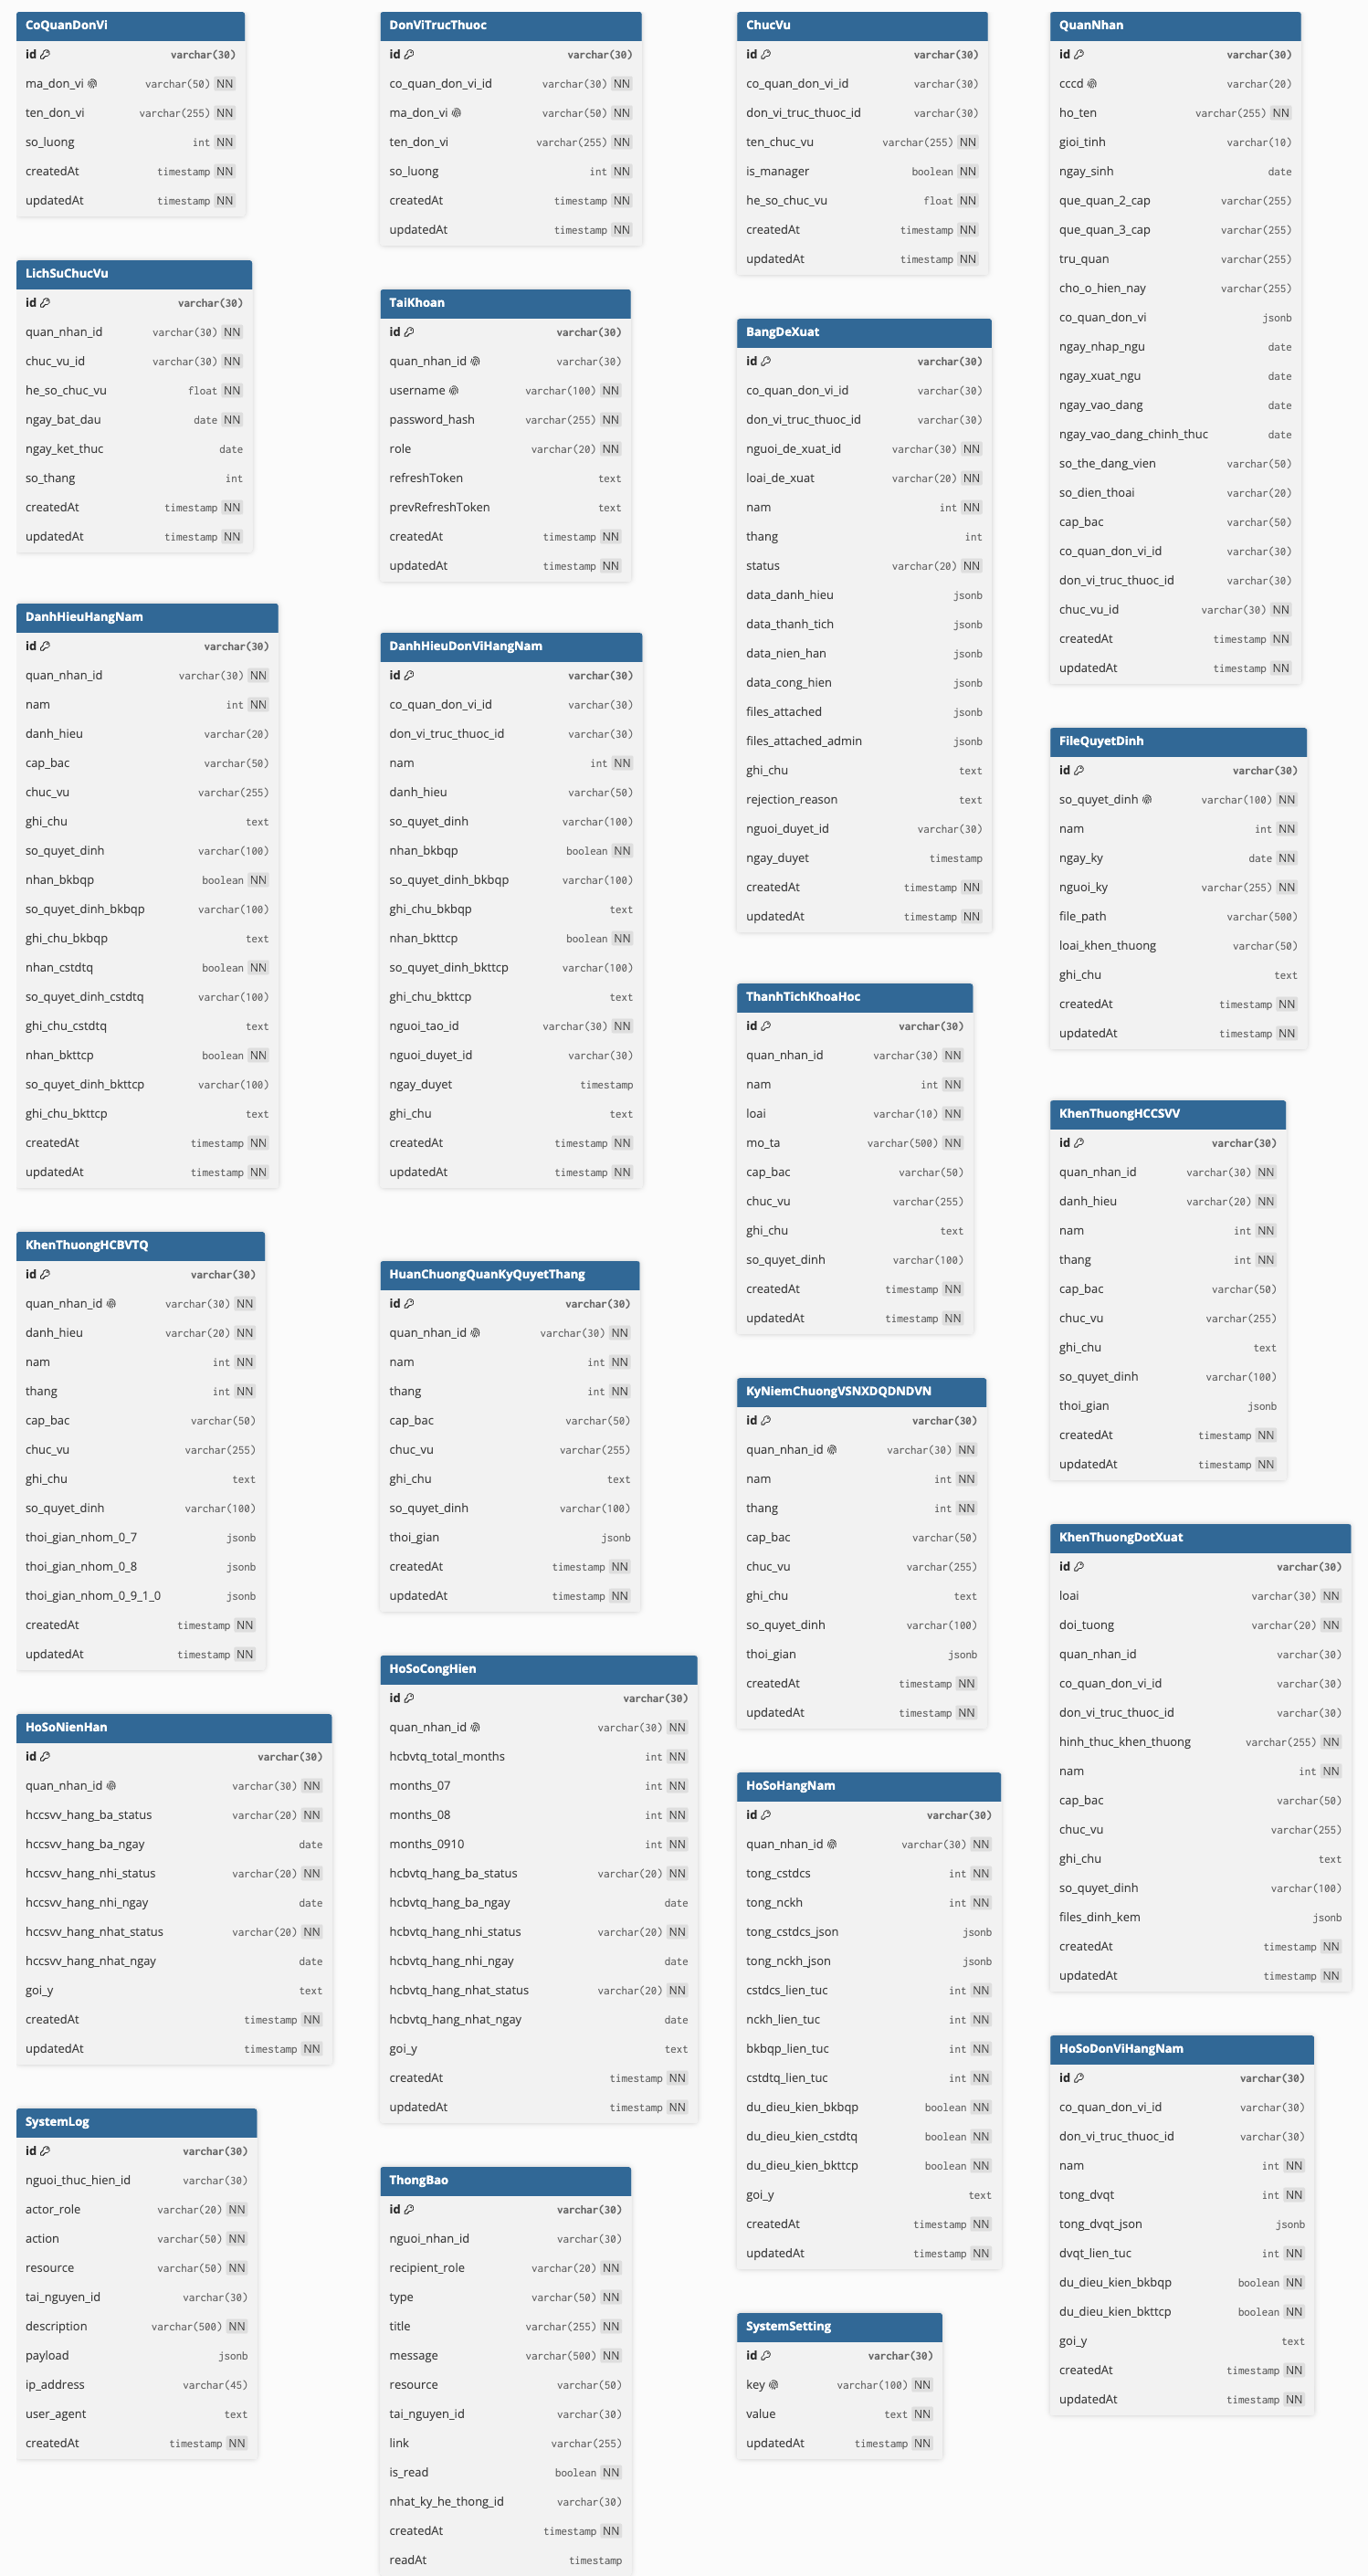
\includegraphics[width=0.9\textwidth]{erd-0-tat-ca-bang}
\graphicspath{{../../Báo cáo ĐATN/Hinhve/}{../../Báo cáo ĐATN/Hinhve/Database/}}

% --- Metadata ---
\title{Phần mềm Quản lý Khen thưởng}
\subtitle{Tại Học viện Khoa học Quân sự}
\author[Trần Anh Đức]{Sinh viên thực hiện: \textbf{Trần Anh Đức}\\Giảng viên hướng dẫn: \textbf{ThS. Lê Đức Trung}}
\institute[ĐHBKHN]{Trường Công nghệ Thông tin và Truyền thông --- Đại học Bách khoa Hà Nội}
\date{Tháng 5/2026}

% =====================================================================
\begin{document}

% --- Slide 1: Title ---
{
\setbeamertemplate{footline}{}
\begin{frame}[plain]
  \begin{center}
    \vspace{0.5cm}
    {\large \textcolor{hustdark}{ĐẠI HỌC BÁCH KHOA HÀ NỘI}}\\
    {\small \textcolor{textmuted}{Trường Công nghệ Thông tin và Truyền thông}}\\[1.2cm]

    {\Huge \textcolor{hustred}{\textbf{PHẦN MỀM QUẢN LÝ}}}\\[0.3cm]
    {\Huge \textcolor{hustred}{\textbf{KHEN THƯỞNG}}}\\[0.5cm]

    {\large Đồ án Tốt nghiệp Đại học --- Niên khóa 2025/2026}\\[1cm]

    \begin{tabular}{rl}
      \textbf{Sinh viên thực hiện} & : Trần Anh Đức \\
      \textbf{Mã số sinh viên} & : 20220120 \\
      \textbf{Giảng viên hướng dẫn} & : ThS. Lê Đức Trung \\
    \end{tabular}\\[0.6cm]

    {\small \textcolor{textmuted}{Hà Nội, tháng 5 năm 2026}}
  \end{center}
\end{frame}
}

% --- Slide 2: Nội dung trình bày ---
\begin{frame}{Nội dung trình bày}
  \begin{columns}[T,onlytextwidth]
    \column{0.5\textwidth}
    \small
    \textcolor{hustdark}{\textbf{Phần I --- Mở đầu}}
    \begin{enumerate}
      \item Mục tiêu của đồ án
      \item Hệ thống khen thưởng
      \item Chuỗi danh hiệu \& các danh hiệu dài hạn
      \item Thách thức \& yêu cầu
    \end{enumerate}
    \vspace{0.05cm}
    \textcolor{hustdark}{\textbf{Phần II --- Công nghệ \& Thiết kế}}
    \begin{enumerate}\setcounter{enumi}{4}
      \item Công nghệ sử dụng
      \item Kiến trúc hệ thống
      \item Cơ sở dữ liệu
      \item Use-case \& quy trình duyệt
      \item Kiến trúc phần mềm (Strategy)
    \end{enumerate}

    \column{0.5\textwidth}
    \small
    \textcolor{hustdark}{\textbf{Phần III --- Các đóng góp nổi bật}}
    \begin{enumerate}\setcounter{enumi}{9}
      \item Tự động xét điều kiện \& gợi ý
      \item Số hoá quy trình \& lưu vết
      \item Nhập Excel có giao dịch
      \item Lưu vết, sao lưu \& thông báo
    \end{enumerate}
    \vspace{0.05cm}
    \textcolor{hustdark}{\textbf{Phần IV --- Đánh giá \& Tổng kết}}
    \begin{enumerate}\setcounter{enumi}{13}
      \item Kiểm thử \& triển khai
      \item Kết luận \& hướng phát triển
    \end{enumerate}
  \end{columns}
\end{frame}

% --- Slide 3: Mục tiêu của đồ án ---
\begin{frame}{Mục tiêu của đồ án}
  \begin{columns}[T,onlytextwidth]
    \column{0.5\textwidth}
    \textbf{Bối cảnh và động lực}
    \begin{itemize}\small
      \item Quản lý khen thưởng tại đơn vị quân đội hiện chủ yếu dựa trên \textbf{Excel và hồ sơ giấy}
      \item Khó tra cứu lịch sử khen thưởng nhiều năm
      \item \highlight{Quy định chuỗi danh hiệu phức tạp} (BKBTBQP, CSTĐTQ, BKTTCP) dễ sai sót khi tính thủ công
      \item Vận hành trên \textbf{mạng nội bộ}, không phụ thuộc Internet
    \end{itemize}

    \column{0.5\textwidth}
    \textbf{Mục tiêu cụ thể}
    \begin{itemize}\small
      \item Quản lý \textbf{bảy nhóm khen thưởng} với 4 cấp vai trò
      \item \textbf{Tự động hoá} xét điều kiện theo quy định hiện hành
      \item Hỗ trợ \textbf{đề xuất $\to$ đính kèm quyết định $\to$ phê duyệt}
      \item Đảm bảo \textbf{truy vết và bảo mật} đầy đủ
      \item \textbf{Triển khai trên mạng nội bộ} offline
    \end{itemize}
    \begin{block}{Mục tiêu cốt lõi}
      \small Giảm sai sót thủ công, tiết kiệm thời gian, đảm bảo đúng quy định.
    \end{block}
  \end{columns}
\end{frame}

% --- Slide 5: Hệ thống khen thưởng — bảy nhóm / loại đề xuất ---
\begin{frame}{Hệ thống khen thưởng}
  \scriptsize
  \begin{tabularx}{\textwidth}{|>{\raggedright\arraybackslash}p{2.8cm}|>{\raggedright\arraybackslash}X|>{\raggedright\arraybackslash}p{2.6cm}|}
    \hline
    \rowcolor{hustred}\textcolor{white}{\textbf{Nhóm khen thưởng}} & \textcolor{white}{\textbf{Phân rã chi tiết}} & \textcolor{white}{\textbf{Tiêu chí xét}} \\ \hline
    \textbf{Khen thưởng hằng năm} & Cá nhân (CSTĐCS, CSTT, BKBTBQP, CSTĐTQ, BKTTCP) + Đơn vị (ĐVQT, ĐVTT, BKBTBQP, BKTTCP) & Theo năm \\ \hline
    \textbf{Khen thưởng niên hạn} & HCCSVV (3 hạng), HCQKQT, KNC VSNXD QĐNDVN & Theo thời gian phục vụ \\ \hline
    \textbf{Khen thưởng cống hiến} & HCBVTQ (3 hạng) & 120 tháng (nam) / 80 (nữ) theo nhóm hệ số \\ \hline
    \textbf{Khen thưởng thành tích} & NCKH (Đề tài KH, Sáng kiến KH) & Theo công trình \\ \hline
    \textbf{Khen thưởng đột xuất} & Theo sự kiện / chiến công cụ thể & Phi định kỳ \\ \hline
  \end{tabularx}

  \vspace{0.4cm}
  \begin{block}{}
    Bốn nhóm đầu gồm \highlight{bảy loại đề xuất} xử lý qua \highlight{Strategy pattern} (phần Kiến trúc phần mềm); khen thưởng đột xuất được quản lý riêng, ngoài luồng đề xuất.
  \end{block}
\end{frame}

% --- Slide 6: Khen thưởng hằng năm — cá nhân + đơn vị (timeline) ⭐ ---
\begin{frame}{Khen thưởng hằng năm --- vòng đời chuỗi danh hiệu}
  \centering

  % ===== CÁ NHÂN lane =====
  \begin{flushleft}\hspace{0.2cm}\textbf{\textcolor{hustdark}{Cá nhân}} \textit{\scriptsize(CSTĐCS + NCKH liên tục mỗi năm là nền tảng; đề xuất chuỗi xét dựa trên streak năm trước)}\end{flushleft}
  \vspace{-0.15cm}
  \begin{tikzpicture}[
    every node/.style={font=\scriptsize},
    base/.style={draw=hustred!60, fill=hustred!5, rounded corners=1pt, font=\tiny, inner sep=1.5pt, align=center},
    award/.style={draw=hustred, fill=hustred!10, rounded corners=2pt, font=\tiny, inner sep=2pt, align=center},
    awardhigh/.style={draw=hustdark, fill=hustred!25, rounded corners=2pt, font=\tiny\bfseries, inner sep=2pt, align=center},
    awardtop/.style={draw=hustdark, fill=hustdark, text=white, rounded corners=3pt, font=\tiny\bfseries, inner sep=2pt, align=center},
    yearmark/.style={draw=hustdark, thick}
  ]
    \draw[->, very thick, hustdark] (-0.3,0) -- (10.0,0);
    \foreach \i in {1,...,8} {
      \pgfmathsetmacro\xcoord{(\i-1)*1.15}
      \draw[yearmark] (\xcoord, 0.08) -- (\xcoord, -0.08);
      \node[above=0.05cm, font=\tiny\bfseries] at (\xcoord, 0.08) {Năm \i};
      \node[base, anchor=north] at (\xcoord, -0.18) {CSTĐCS};
    }
    \node[right, font=\tiny] at (10.0, -0.05) {\dots};

    % Năm 3: BKBTBQP#1
    \node[award, anchor=south] (b1) at (2.30, 0.65) {BKBTBQP \#1};
    \draw[hustred, dashed, thin] (2.30, 0.5) -- (b1.south);

    % Năm 4: CSTĐTQ#1
    \node[awardhigh, anchor=south] (c1) at (3.45, 1.3) {CSTĐTQ \#1};
    \draw[hustdark, dashed, thin] (3.45, 0.5) -- (c1.south);

    % Năm 5: BKBTBQP#2
    \node[award, anchor=south] (b2) at (4.60, 0.65) {BKBTBQP \#2};
    \draw[hustred, dashed, thin] (4.60, 0.5) -- (b2.south);

    % Năm 7: BKBTBQP#3 + CSTĐTQ#2
    \node[awardhigh, anchor=south] (c2) at (6.90, 1.3) {BKBTBQP \#3 + CSTĐTQ \#2};
    \draw[hustdark, dashed, thin] (6.90, 0.5) -- (c2.south);

    % Năm 8: BKTTCP
    \node[awardtop, anchor=south] (bk) at (8.05, 2.0) {$\bigstar$ BKTTCP (một lần)};
    \draw[hustdark, very thick] (8.05, 0.5) -- (bk.south);
  \end{tikzpicture}

  \vspace{0.1cm}

  % ===== ĐƠN VỊ lane =====
  \begin{flushleft}\hspace{0.2cm}\textbf{\textcolor{hustdark}{Đơn vị}} \textit{\scriptsize(ĐVQT liên tục; không CSTĐTQ, không bắt buộc NCKH, BKTTCP lặp lại)}\end{flushleft}
  \vspace{-0.15cm}
  \begin{tikzpicture}[
    every node/.style={font=\scriptsize},
    base/.style={draw=hustred!60, fill=hustred!5, rounded corners=1pt, font=\tiny, inner sep=1.5pt, align=center},
    uaward/.style={draw=hustred, fill=hustred!10, rounded corners=2pt, font=\tiny, inner sep=2pt, align=center},
    uawardtop/.style={draw=hustdark, fill=hustred!40, rounded corners=3pt, font=\tiny\bfseries, inner sep=2pt, align=center},
    yearmark/.style={draw=hustdark, thick}
  ]
    \draw[->, very thick, hustdark] (-0.3,0) -- (10.0,0);
    \foreach \i in {1,...,8} {
      \pgfmathsetmacro\xcoord{(\i-1)*1.15}
      \draw[yearmark] (\xcoord, 0.08) -- (\xcoord, -0.08);
      \node[above=0.05cm, font=\tiny\bfseries] at (\xcoord, 0.08) {Năm \i};
      \node[base, anchor=north] at (\xcoord, -0.18) {ĐVQT};
    }
    \node[right, font=\tiny] at (10.0, -0.05) {\dots\ \textit{(lặp lại)}};

    % Năm 3, 5, 7: BKBTBQP đv
    \node[uaward, anchor=south] (ub1) at (2.30, 0.65) {BKBTBQP đv \#1};
    \draw[hustred, dashed, thin] (2.30, 0.5) -- (ub1.south);

    \node[uaward, anchor=south] (ub2) at (4.60, 0.65) {BKBTBQP đv \#2};
    \draw[hustred, dashed, thin] (4.60, 0.5) -- (ub2.south);

    \node[uaward, anchor=south] (ub3) at (6.90, 0.65) {BKBTBQP đv \#3};
    \draw[hustred, dashed, thin] (6.90, 0.5) -- (ub3.south);

    % Năm 8: BKTTCP đv
    \node[uawardtop, anchor=south] (ubk) at (8.05, 1.3) {BKTTCP đv \\ (lặp lại)};
    \draw[hustdark, very thick] (8.05, 0.5) -- (ubk.south);
  \end{tikzpicture}

  \vspace{-0.1cm}
  \scriptsize\centering
  \textcolor{hustdark}{\textbf{Lỡ đợt:}} bỏ lỡ năm đến mốc thì chu kỳ vẫn đếm tiếp, chu kỳ sau vẫn được xét.
\end{frame}

% --- Slide 7: Các loại khen thưởng còn lại — niên hạn + 1-lần + cống hiến ⭐ ---
\begin{frame}{Bốn loại khen thưởng dài hạn}
  \begin{columns}[T,onlytextwidth]
    \column{0.58\textwidth}

    \textbf{\textcolor{hustdark}{Niên hạn + 1-lần (theo năm phục vụ)}}\\[0.05cm]
    \begin{tikzpicture}[
      every node/.style={font=\scriptsize},
      nh/.style={draw=hustred, fill=hustred!10, rounded corners=2pt, font=\tiny, inner sep=1.5pt, align=center, minimum width=1.1cm},
      once/.style={draw=hustdark, fill=hustdark, text=white, rounded corners=3pt, font=\tiny\bfseries, inner sep=1.5pt, align=center, minimum width=1.1cm},
      knc/.style={draw=hustdark, fill=hustred!40, rounded corners=3pt, font=\tiny\bfseries, inner sep=1.5pt, align=center, minimum width=1.1cm},
      yearmark/.style={draw=hustdark, thick}
    ]
      \draw[->, very thick, hustdark] (0,0) -- (6.0,0);
      \foreach \i [count=\j from 0] in {10, 15, 20, 25} {
        \pgfmathsetmacro\xcoord{0.4 + \j*1.55}
        \draw[yearmark] (\xcoord, 0.1) -- (\xcoord, -0.1);
        \node[below=0.06cm, font=\tiny\bfseries] at (\xcoord, 0) {Năm \i};
      }

      % Year 10: HCCSVV hạng Ba
      \node[nh, anchor=south] (n1) at (0.4, 0.3) {HCCSVV \\ Ba};
      % Year 15: HCCSVV hạng Nhì
      \node[nh, anchor=south] (n2) at (1.95, 0.3) {HCCSVV \\ Nhì};
      % Year 20: HCCSVV hạng Nhất + KNC nữ
      \node[nh, anchor=south] (n3) at (3.5, 0.3) {HCCSVV \\ Nhất};
      \node[knc, above=0.04cm of n3] (kn) {KNC (nữ)};
      % Year 25: HCQKQT + KNC nam
      \node[knc, anchor=south] (km) at (5.05, 0.3) {KNC (nam)};
      \node[once, above=0.04cm of km] (q) {HCQKQT};

      \draw[hustred, dashed, thin] (0.4, 0.1) -- (n1.south);
      \draw[hustred, dashed, thin] (1.95, 0.1) -- (n2.south);
      \draw[hustred, dashed, thin] (3.5, 0.1) -- (n3.south);
      \draw[hustdark, very thick] (5.05, 0.1) -- (km.south);
    \end{tikzpicture}

    \vspace{0.15cm}
    \scriptsize
    \textbf{HCCSVV} 3 hạng theo mốc 10/15/20y. \textbf{HCQKQT} 25y --- 1 lần.\\
    \textbf{KNC VSNXD QĐNDVN}: nam 25y / nữ 20y --- 1 lần duy nhất.

    \column{0.42\textwidth}

    \textbf{\textcolor{hustdark}{Cống hiến (HCBVTQ)}}\\[0.05cm]
    \scriptsize Tích luỹ \textbf{120 tháng} (nam) hoặc \textbf{80 tháng} (nữ, bằng 2/3) giữ chức vụ trong từng \emph{nhóm hệ số chức vụ}, không phụ thuộc số năm phục vụ:\\[0.15cm]

    \begin{tikzpicture}[
      every node/.style={font=\tiny},
      grpbox/.style={draw=hustred, fill=hustred!10, rounded corners=2pt, inner sep=3pt, minimum width=1.6cm, font=\tiny\bfseries, align=center},
      tierbox/.style={draw=hustdark, fill=hustred!30, rounded corners=2pt, inner sep=3pt, minimum width=1.4cm, font=\tiny\bfseries, align=center}
    ]
      % Row 1: nhóm 0.7 → Hạng Ba
      \node[grpbox] (g1) at (0,0) {Nhóm 0.7};
      \node[tierbox] (t1) at (3.4,0) {Hạng Ba};
      \draw[->, thick, hustdark] (g1.east) -- node[above, font=\tiny]{120 tháng} (t1.west);

      % Row 2: nhóm 0.8 → Hạng Nhì
      \node[grpbox] (g2) at (0,-0.9) {Nhóm 0.8};
      \node[tierbox] (t2) at (3.4,-0.9) {Hạng Nhì};
      \draw[->, thick, hustdark] (g2.east) -- node[above, font=\tiny]{120 tháng} (t2.west);

      % Row 3: nhóm 0.9-1.0 → Hạng Nhất
      \node[grpbox] (g3) at (0,-1.8) {Nhóm 0.9--1.0};
      \node[tierbox] (t3) at (3.4,-1.8) {Hạng Nhất};
      \draw[->, thick, hustdark] (g3.east) -- node[above, font=\tiny]{120 tháng} (t3.west);
    \end{tikzpicture}
  \end{columns}
\end{frame}

% --- Phân tích bài toán: bốn thách thức cốt lõi ---
\begin{frame}{Phân tích bài toán --- bốn thách thức cốt lõi}
  \begin{columns}[T,onlytextwidth]
    \column{0.5\textwidth}
    \textbf{\textcolor{hustred}{\textcircled{1} Logic chuỗi danh hiệu nhiều năm}}\\
    \scriptsize Cửa sổ trượt 3 năm và 7 năm, ràng buộc nhận một lần duy nhất và tình huống lỡ đợt khiến không thể xét bằng một truy vấn đơn lẻ; phải xét trên toàn dòng thời gian của quân nhân.\\[0.3cm]

    \textbf{\textcolor{hustred}{\textcircled{2} Tính nhất quán đa bảng}}\\
    \scriptsize Mỗi lần duyệt đề xuất cập nhật nhiều bảng cùng lúc (đề xuất, hồ sơ, quyết định, thông báo, nhật ký), nên bắt buộc dùng giao dịch và chống tranh chấp ghi khi hai cán bộ duyệt cùng lúc.

    \column{0.5\textwidth}
    \textbf{\textcolor{hustred}{\textcircled{3} Phân quyền theo cây tổ chức}}\\
    \scriptsize Bốn vai trò trên cây đơn vị nhiều cấp đòi hỏi hai lớp middleware độc lập (kiểm tra vai trò và lọc theo đơn vị); bypass được lớp này thì lớp kia vẫn chặn.\\[0.3cm]

    \textbf{\textcolor{hustred}{\textcircled{4} Vận hành trong mạng nội bộ}}\\
    \scriptsize Không có Internet hay dịch vụ ngoài, nên hệ thống tự lưu trữ phông chữ, tự sao lưu theo lịch và tự khởi động lại bằng PM2.
  \end{columns}

  \vspace{0.4cm}
  \begin{block}{}
    \centering\small Trọng tâm là hai thách thức \textcircled{1} và \textcircled{2}; các đóng góp ở phần sau giải quyết trực tiếp hai vấn đề này.
  \end{block}
\end{frame}

% --- Công nghệ sử dụng ---
\begin{frame}{Công nghệ sử dụng --- Tech Stack}
  \begin{columns}[T,onlytextwidth]
    \column{0.5\textwidth}
    \textcolor{hustred}{\textbf{Frontend}}
    \begin{itemize}\small
      \item \textbf{Next.js} (App Router) --- server components, file-based routing
      \item \textbf{TypeScript} --- type safety toàn dự án
      \item \textbf{Ant Design} --- component nghiệp vụ (Form, Table, DatePicker, Modal, ...)
      \item \textbf{Tailwind CSS} --- styling tuỳ biến cho layout, spacing
      \item \textbf{Zod} --- schema validation chia sẻ giữa client và server
      \item \textbf{Socket.IO client} --- nhận thông báo real-time
    \end{itemize}

    \column{0.5\textwidth}
    \textcolor{hustred}{\textbf{Backend \& CSDL}}
    \begin{itemize}\small
      \item \textbf{Express + TypeScript} --- REST API
      \item \textbf{Prisma ORM} --- type-safe queries, migration tự động
      \item \textbf{PostgreSQL} --- RDBMS, giao dịch ACID đa bảng
      \item \textbf{Zod} --- validate hai tầng (BE + FE) cùng phong cách schema
      \item \textbf{JWT 2 token} --- access + refresh
      \item \textbf{bcrypt} --- hash password
    \end{itemize}
  \end{columns}

  \vspace{0.3cm}
  \centering
  \hustpill{Socket.IO} \hustpill{PM2} \hustpill{node-cron} \hustpill{ExcelJS} \hustpill{Multer} \hustpill{Helmet} \hustpill{Local deploy}
\end{frame}

% --- Slide 8: Kiến trúc tổng quan ---
\begin{frame}{Kiến trúc tổng quan hệ thống}
  \centering
  \begin{block}{Luồng dữ liệu chính}
    \centering\small
    \textcolor{hustred}{\textbf{Trình duyệt}} $\xrightarrow{\text{HTTPS}}$ \textcolor{hustred}{\textbf{Frontend (Next.js)}} \;\textit{\footnotesize tải giao diện}\\[0.25cm]
    \textcolor{hustred}{\textbf{Trình duyệt}} $\xrightarrow{\text{REST\,/\,Socket.IO}}$ \textcolor{hustred}{\textbf{Backend (Express)}} $\xrightarrow{\text{Prisma}}$ \textcolor{hustred}{\textbf{PostgreSQL}}\\[0.15cm]
    \footnotesize \textcolor{hustdark}{\textit{Trình duyệt gọi trực tiếp Backend qua REST API và Socket.IO, không đi qua Frontend.}}
  \end{block}

  \vspace{0.1cm}
  \centering
  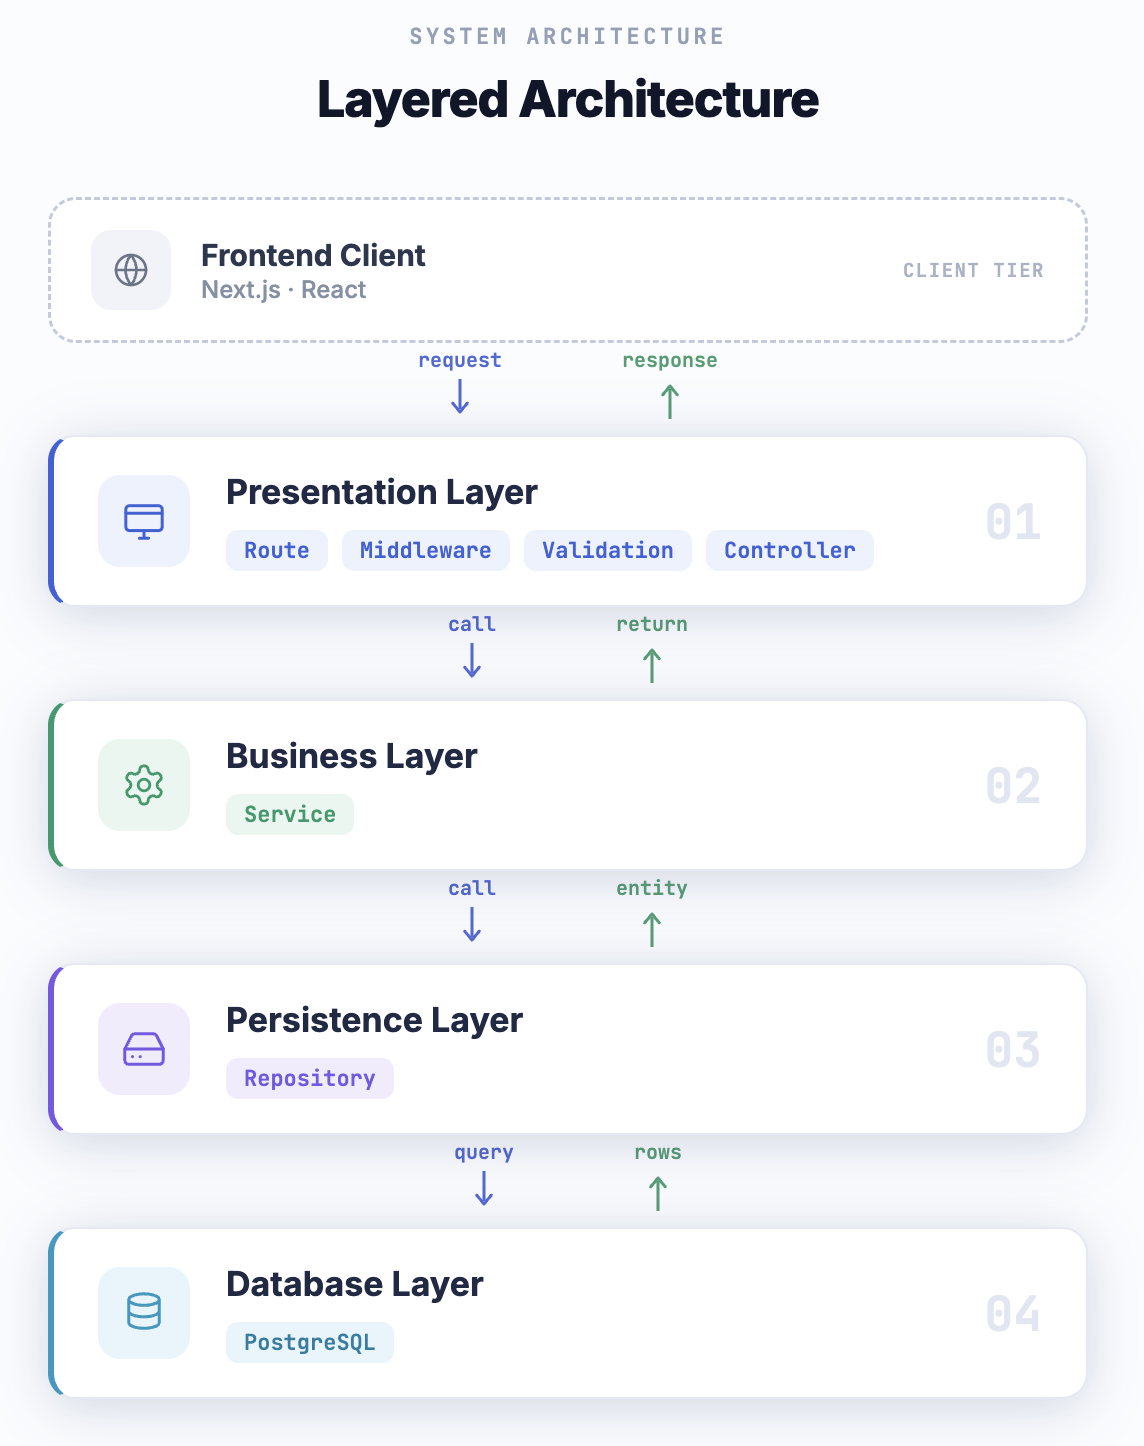
\includegraphics[width=\textwidth,height=0.5\textheight,keepaspectratio]{KienTrucPhanTang}
\end{frame}

% --- Slide 10: Thiết kế CSDL ---
\begin{frame}{Thiết kế cơ sở dữ liệu}
  \begin{columns}[T,onlytextwidth]
    \column{0.5\textwidth}
    \textbf{Tổng quan}\\
    \begin{block}{}
      \centering {\LARGE \textcolor{hustred}{\textbf{23}}} bảng, \textbf{47} khoá ngoại, khoá chính kiểu CUID
    \end{block}

    \textbf{Nhóm bảng}
    \begin{itemize}\scriptsize
      \item \textbf{Tổ chức} --- \texttt{QuanNhan}, \texttt{CoQuanDonVi}, \texttt{DonViTrucThuoc}, \texttt{ChucVu}
      \item \textbf{Đề xuất \& Hồ sơ} --- \texttt{BangDeXuat}, \texttt{DanhHieuHangNam}, \texttt{HoSoNienHan}, \texttt{HoSoCongHien}
      \item \textbf{Tài khoản} --- \texttt{TaiKhoan} (4 vai trò)
      \item \textbf{Phụ trợ} --- \texttt{SystemLog}, \texttt{ThongBao}, \texttt{FileQuyetDinh}, \texttt{SystemSetting}
    \end{itemize}

    \column{0.5\textwidth}
    \begin{block}{Điểm thiết kế đặc biệt}
      \scriptsize
      \texttt{FileQuyetDinh} liên kết với 8 bảng khen thưởng qua \textbf{khoá ngoại theo số quyết định} (khoá tự nhiên, không dùng ID surrogate).\\[0.2cm]
      PostgreSQL tự cascade khi đổi số quyết định, đảm bảo toàn vẹn ở tầng cơ sở dữ liệu.
    \end{block}

    \textbf{Composite uniques}
    \begin{itemize}\scriptsize
      \item \texttt{\scriptsize DanhHieuHangNam}\\\hspace*{0.3cm}\texttt{\scriptsize (quan\_nhan\_id, nam)}
      \item \texttt{\scriptsize KhenThuongHCCSVV}\\\hspace*{0.3cm}\texttt{\scriptsize (quan\_nhan\_id, danh\_hieu)}
      \item \texttt{\scriptsize ChucVu}\\\hspace*{0.3cm}\texttt{\scriptsize (co\_quan\_don\_vi\_id, ten\_chuc\_vu)}
    \end{itemize}
  \end{columns}
\end{frame}

% --- ERD tổng quan ---
\begin{frame}{Thiết kế cơ sở dữ liệu --- Sơ đồ ERD tổng quan}
  \centering
  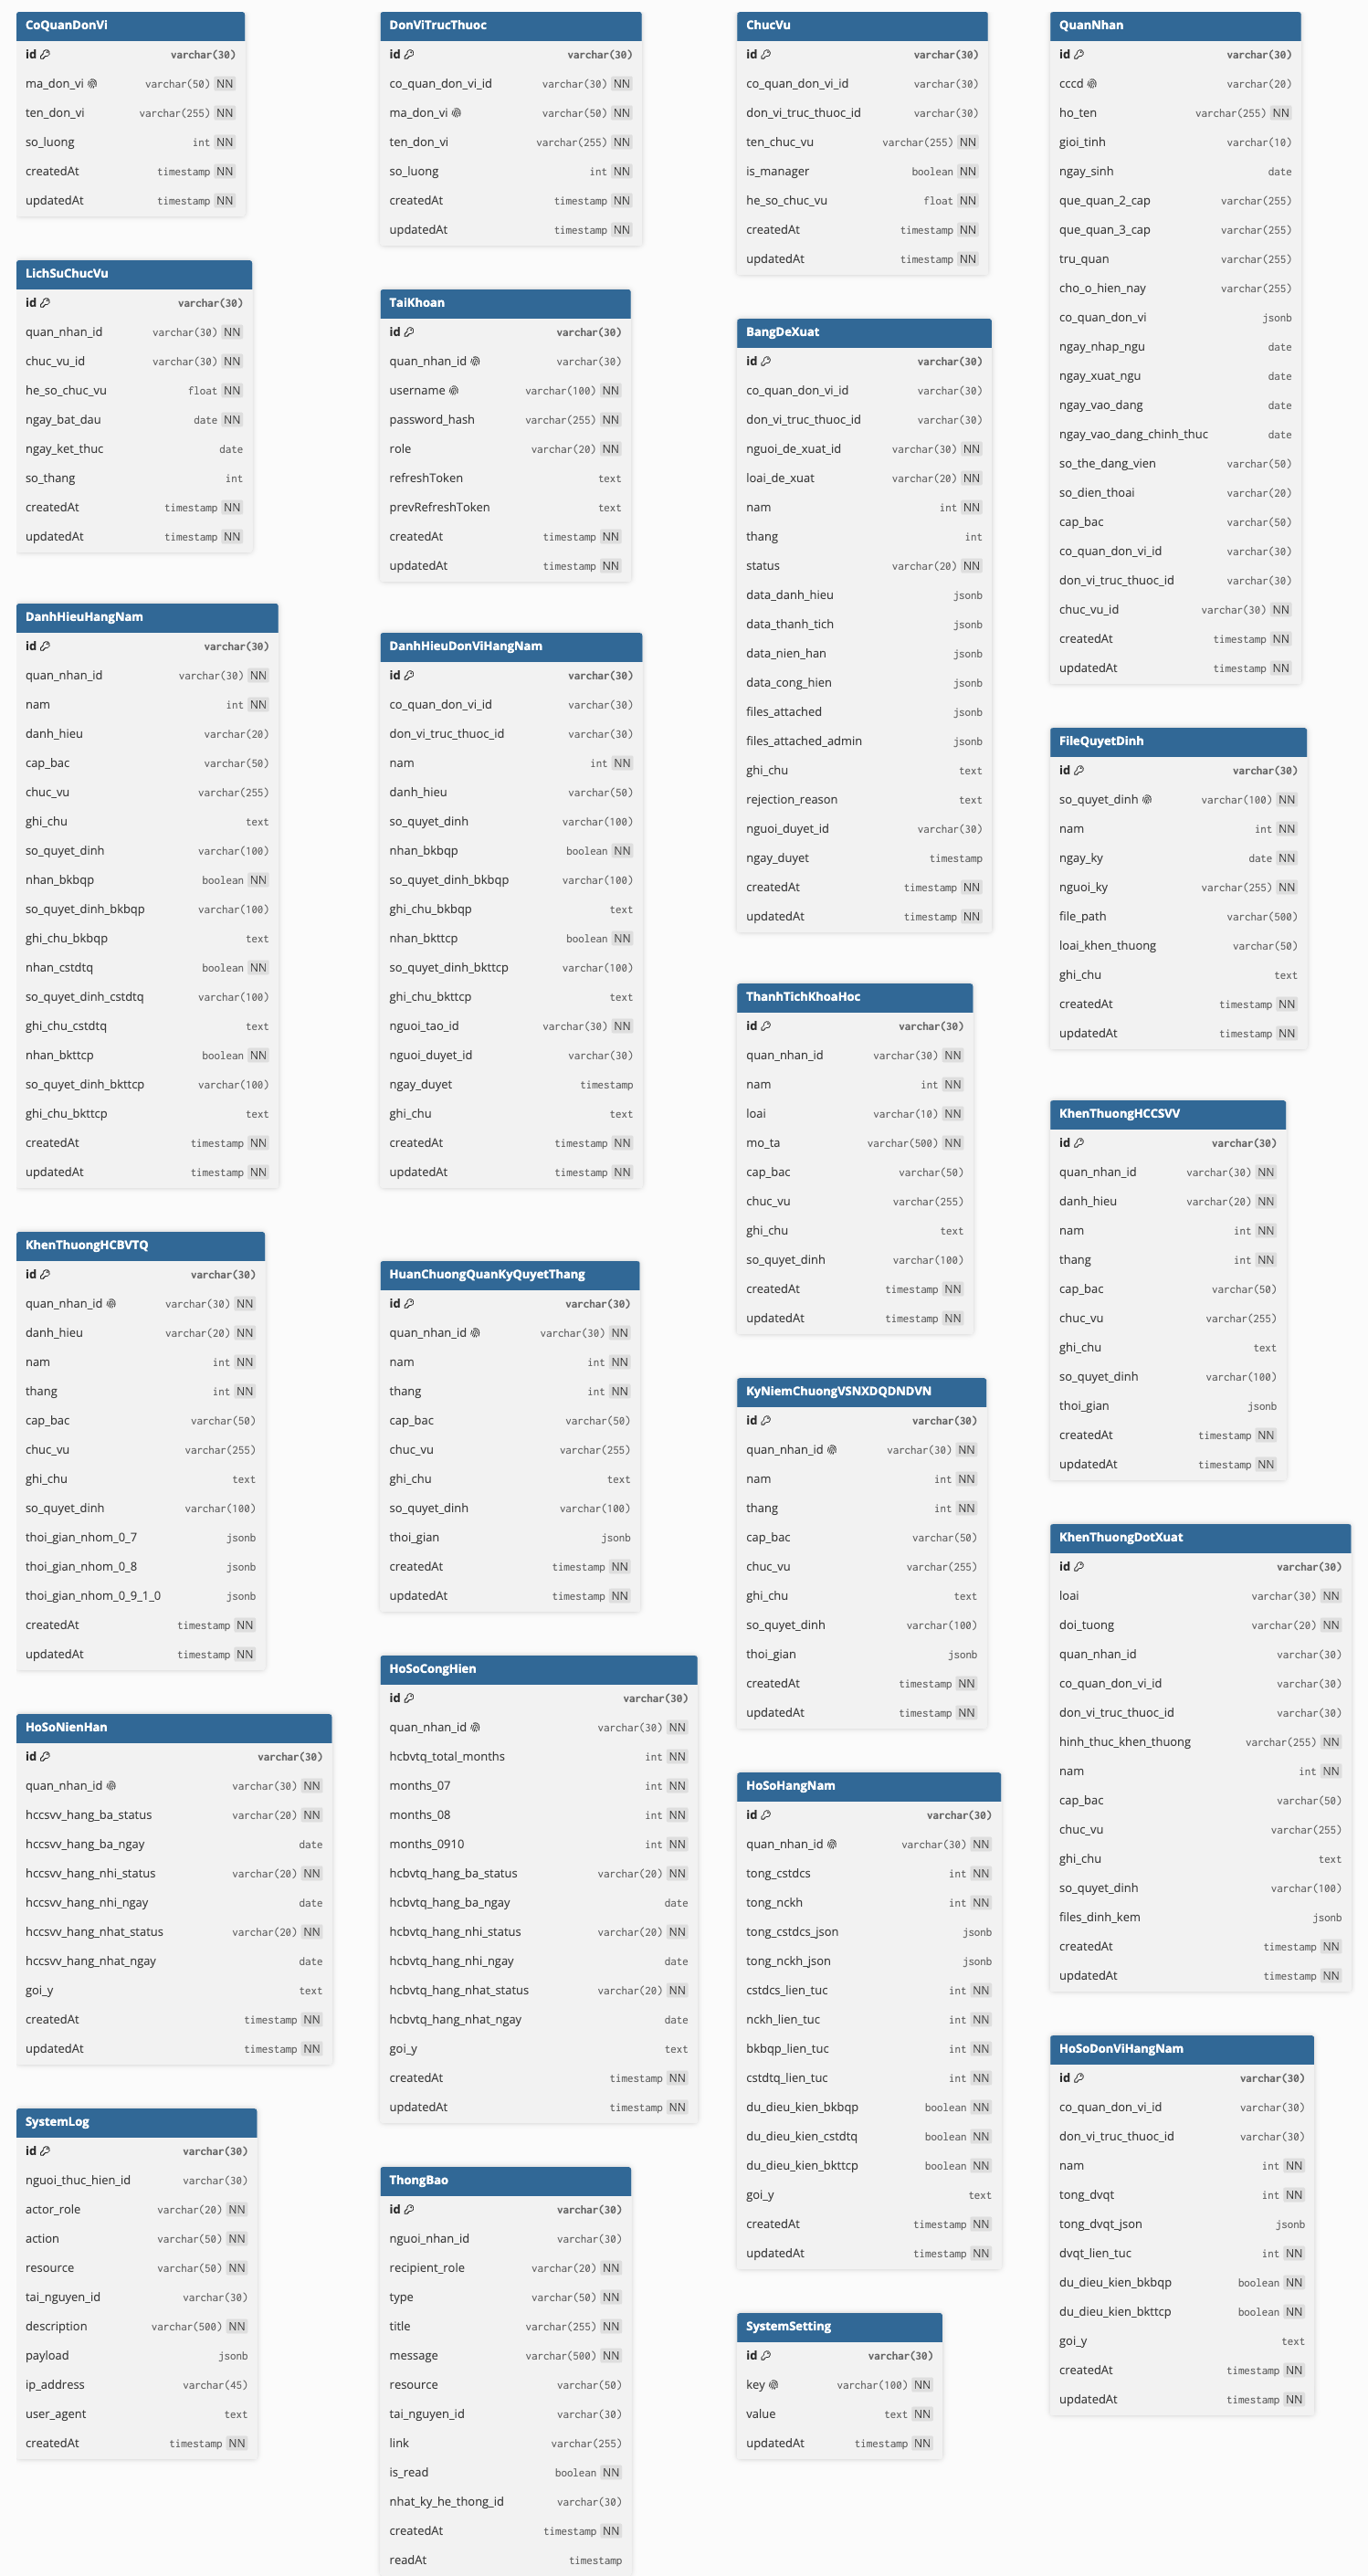
\includegraphics[width=\textwidth,height=0.78\textheight,keepaspectratio]{erd-0-tat-ca-bang}\\[0.1cm]
  {\scriptsize 23 bảng, 47 khoá ngoại, chia thành sáu nhóm dữ liệu nghiệp vụ; quan hệ chi tiết từng nhóm ở các slide tiếp theo.}
\end{frame}

% --- Slide 11: Use-case Diagram ---
\begin{frame}{Phân tích chức năng --- Use-case Diagram}
  \setlength{\tabcolsep}{3.5pt}%
  \begin{columns}[T,onlytextwidth]
    \column{0.42\textwidth}
    \textbf{Phân quyền theo vai trò}\\[0.2cm]
    \scriptsize
    \begin{tabular}{|>{\raggedright\arraybackslash}p{2.5cm}|>{\raggedright\arraybackslash}p{1.9cm}|}
      \hline
      \rowcolor{hustred}\textcolor{white}{\textbf{Vai trò}} & \textcolor{white}{\textbf{Phạm vi}} \\ \hline
      \textbf{Quản trị hệ thống} & Hạ tầng, quản trị \\ \hline
      \textbf{Cán bộ Phòng Chính trị} & Toàn nghiệp vụ \\ \hline
      \textbf{Chỉ huy đơn vị} & Đơn vị phụ trách \\ \hline
      \textbf{Người dùng} & Cá nhân \\ \hline
    \end{tabular}\\[0.3cm]

    \begin{block}{Hai lớp phân quyền}
      \scriptsize
      Một middleware kiểm tra vai trò chặn ở route, một middleware lọc dữ liệu theo đơn vị --- hai lớp độc lập, bypass được lớp này thì lớp kia vẫn chặn.
    \end{block}

    \column{0.55\textwidth}
    \textbf{Use-case chính theo vai trò}\\[0.2cm]
    \scriptsize
    \begin{tabular}{|>{\raggedright\arraybackslash}p{2.4cm}|>{\raggedright\arraybackslash}p{3.2cm}|}
      \hline
      \rowcolor{hustdark}\textcolor{white}{\textbf{Vai trò}} & \textcolor{white}{\textbf{Use-case chính}} \\ \hline
      Quản trị hệ thống & Quản trị hệ thống, sao lưu, nhật ký toàn hệ thống \\ \hline
      Cán bộ Phòng Chính trị & Duyệt đề xuất, nhập số quyết định, quản lý quân nhân \\ \hline
      Chỉ huy đơn vị & Tạo đề xuất, xem hồ sơ đơn vị, tính lại hồ sơ quân nhân \\ \hline
      Người dùng & Xem hồ sơ cá nhân, nhận thông báo \\ \hline
    \end{tabular}
  \end{columns}
\end{frame}

% --- ERD nhóm 1 ---
\begin{frame}{ERD --- Tổ chức, Quân nhân, Tài khoản}
  \centering
  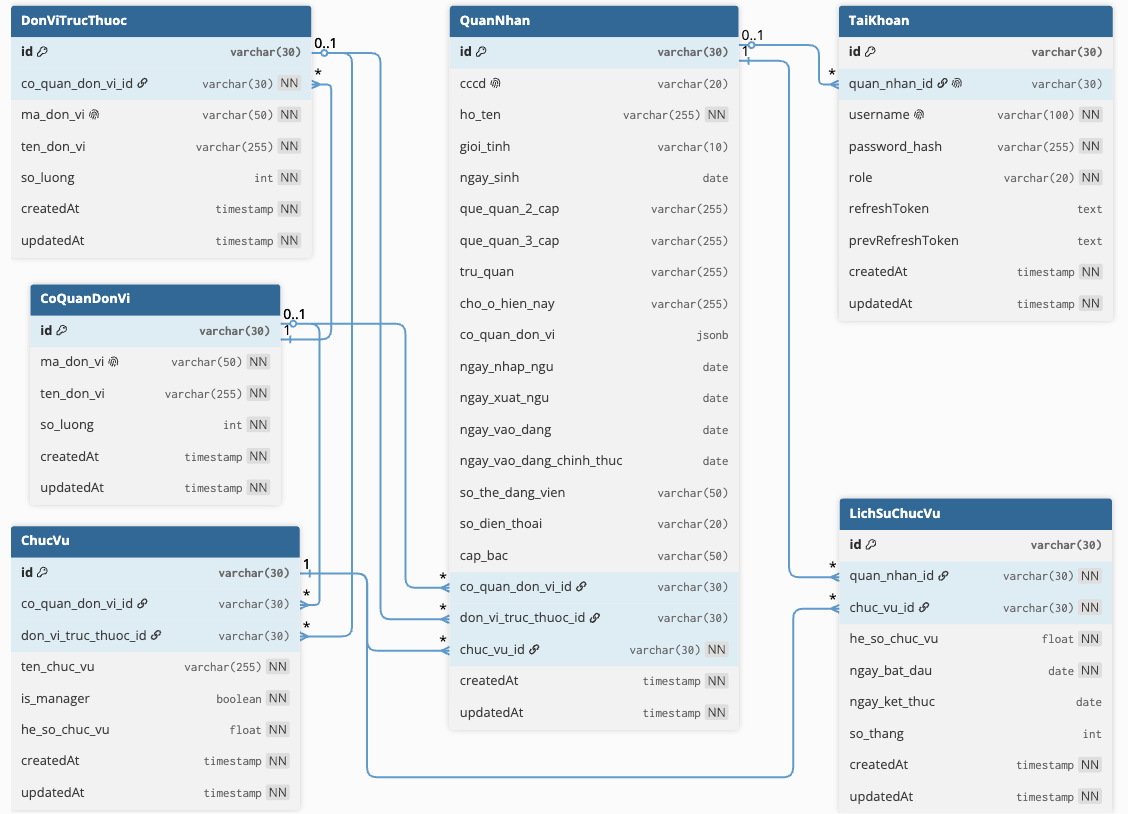
\includegraphics[width=\textwidth,height=0.46\textheight,keepaspectratio]{erd-1-to-chuc}\\[0.05cm]
  \scriptsize\raggedright \textbf{Sáu bảng, chín khoá ngoại.} Quan hệ chính:
  \begin{itemize}\scriptsize
    \item Một \texttt{CoQuanDonVi} có nhiều \texttt{DonViTrucThuoc}.
    \item Mỗi \texttt{QuanNhan} gắn với một \texttt{ChucVu} và một đơn vị (\texttt{CoQuanDonVi} hoặc \texttt{DonViTrucThuoc}).
    \item Mỗi \texttt{QuanNhan} có tối đa một \texttt{TaiKhoan}; \texttt{LichSuChucVu} ghi nhiều giai đoạn giữ chức vụ của một quân nhân (để tính tháng cống hiến).
    \item \texttt{ChucVu} thuộc một đơn vị, duy nhất theo cặp (đơn vị, tên chức vụ).
  \end{itemize}
\end{frame}

% --- ERD nhóm 2 ---
\begin{frame}{ERD --- Đề xuất khen thưởng}
  \centering
  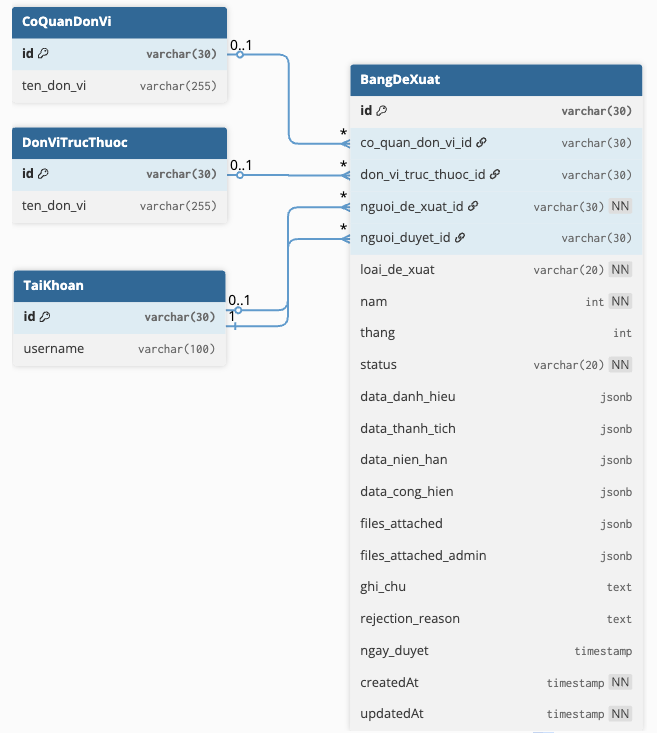
\includegraphics[width=\textwidth,height=0.5\textheight,keepaspectratio]{erd-2-de-xuat}\\[0.05cm]
  \scriptsize\raggedright \textbf{\texttt{BangDeXuat} là trung tâm, bốn khoá ngoại:}
  \begin{itemize}\scriptsize
    \item Mỗi đề xuất gắn với một đơn vị nộp.
    \item Mỗi đề xuất ghi nhận \texttt{TaiKhoan} người đề xuất và \texttt{TaiKhoan} người duyệt.
    \item Không nối trực tiếp tới bảng khen thưởng --- chi tiết từng loại nằm trong các cột JSON (\texttt{data\_danh\_hieu}, \texttt{data\_thanh\_tich}, \texttt{data\_nien\_han}, \texttt{data\_cong\_hien}), chỉ ghi thành bản ghi khen thưởng khi phê duyệt.
  \end{itemize}
\end{frame}

% --- ERD nhóm 3 ---
\begin{frame}{ERD --- Khen thưởng \& hồ sơ cá nhân}
  \centering
  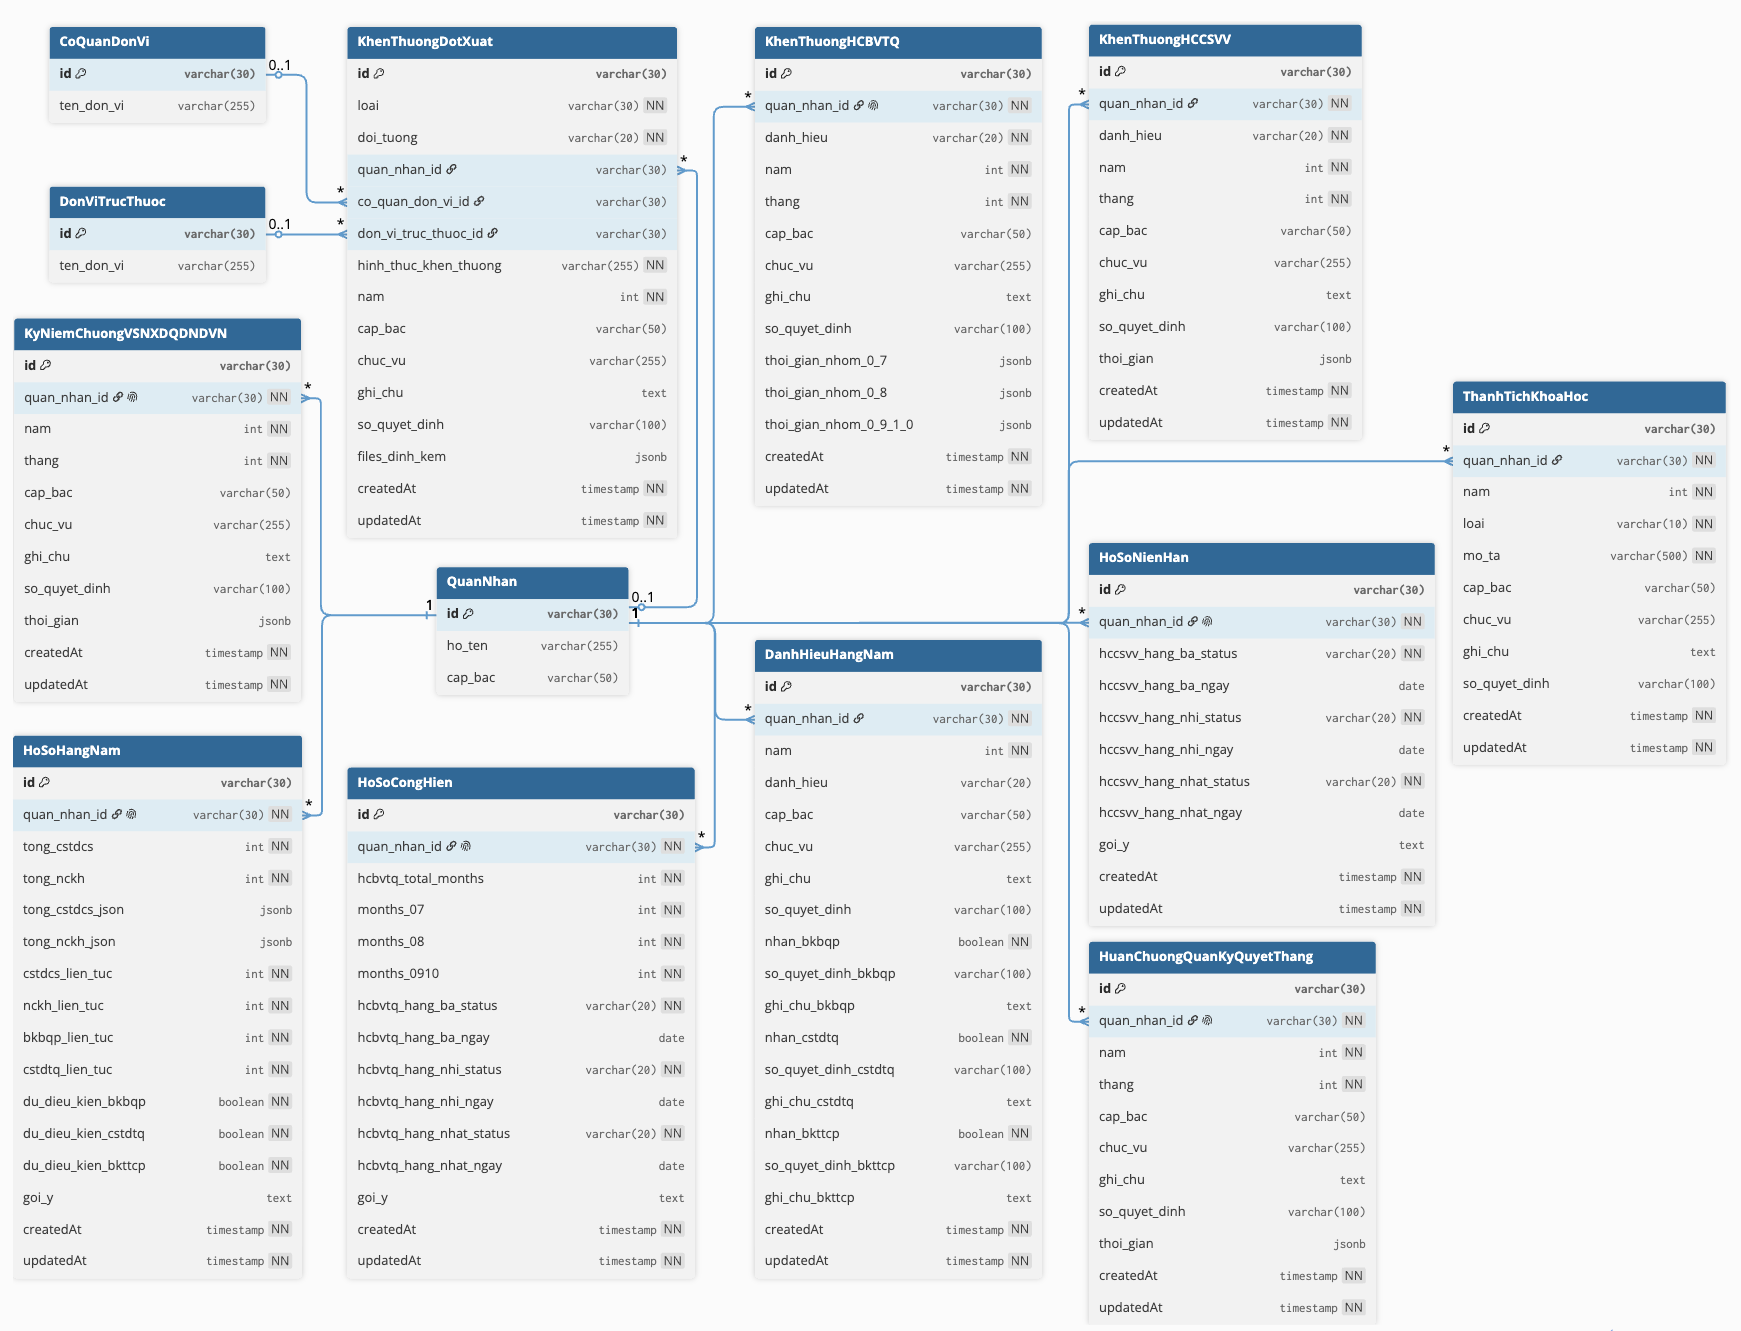
\includegraphics[width=\textwidth,height=0.44\textheight,keepaspectratio]{erd-3-khen-thuong-ca-nhan}\\[0.05cm]
  \scriptsize\raggedright \textbf{Mười bảng, mười hai khoá ngoại tới \texttt{QuanNhan}:}
  \begin{itemize}\scriptsize
    \item Một quân nhân có nhiều bản ghi \texttt{DanhHieuHangNam}, \texttt{ThanhTichKhoaHoc}, \texttt{KhenThuongHCCSVV}.
    \item Mỗi quân nhân chỉ có một bản ghi cho \texttt{HCBVTQ}, \texttt{HCQKQT}, \texttt{KNC} và ba bảng \texttt{HoSo*} (quan hệ một--một).
    \item Mỗi bản ghi tham chiếu một \texttt{FileQuyetDinh} (riêng \texttt{DanhHieuHangNam} tham chiếu bốn lần --- mỗi cấp một số QĐ).
    \item Duy nhất (quân nhân, năm) ở \texttt{DanhHieuHangNam}, (quân nhân, hạng) ở \texttt{HCCSVV}; xoá quân nhân thì các bản ghi xoá theo.
  \end{itemize}
\end{frame}

% --- ERD nhóm 4 ---
\begin{frame}{ERD --- Khen thưởng \& hồ sơ đơn vị}
  \centering
  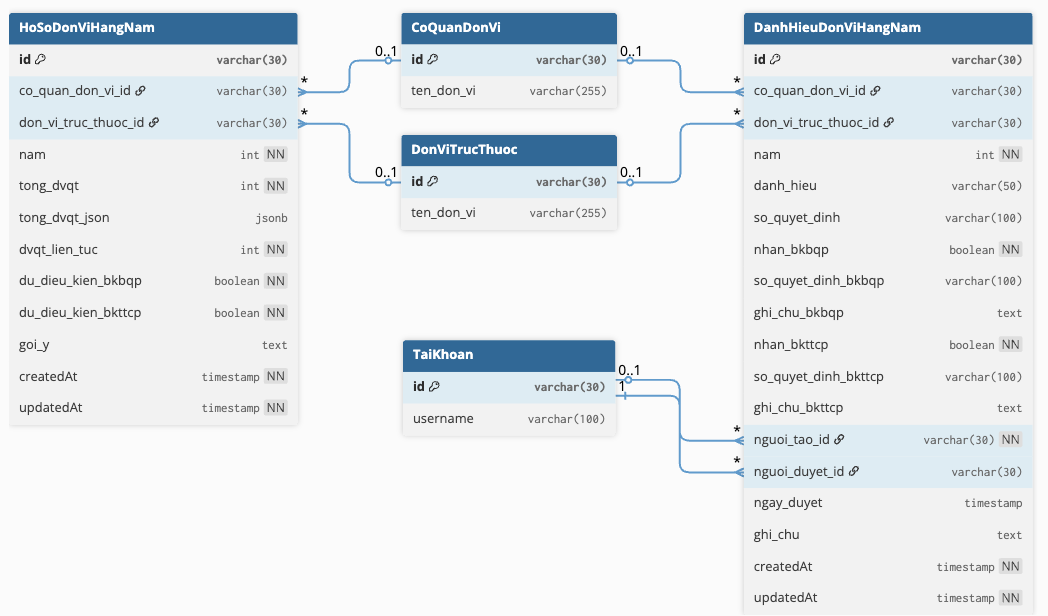
\includegraphics[width=\textwidth,height=0.5\textheight,keepaspectratio]{erd-4-don-vi}\\[0.05cm]
  \scriptsize\raggedright \textbf{Hai bảng, sáu khoá ngoại:}
  \begin{itemize}\scriptsize
    \item Mỗi bản ghi gắn với một đơn vị được khen (\texttt{CoQuanDonVi} hoặc \texttt{DonViTrucThuoc} tuỳ cấp).
    \item \texttt{DanhHieuDonViHangNam} còn ghi nhận \texttt{TaiKhoan} người tạo, người duyệt và tham chiếu \texttt{FileQuyetDinh}.
    \item Duy nhất theo cặp (đơn vị, năm) ở cả hai bảng.
  \end{itemize}
\end{frame}

% --- ERD nhóm 5 ---
\begin{frame}{ERD --- Quyết định}
  \centering
  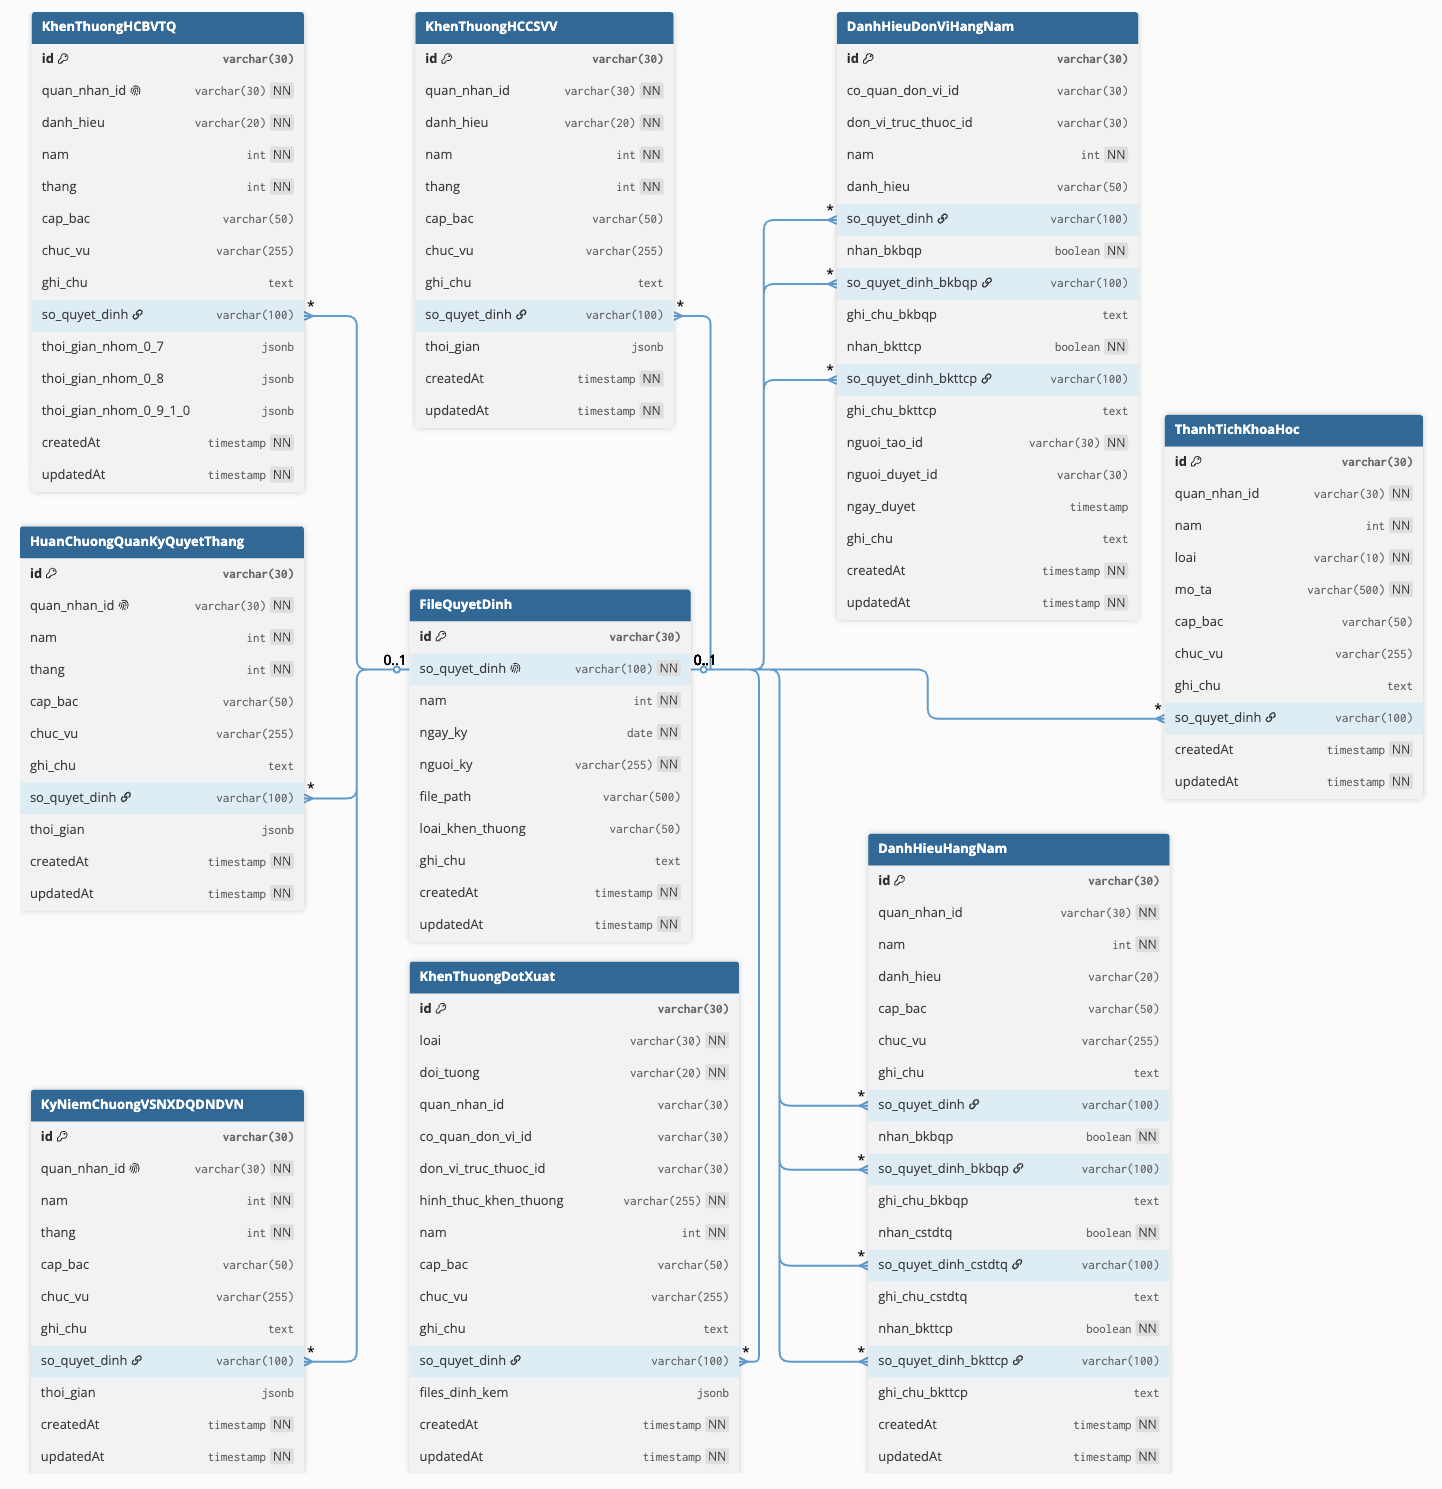
\includegraphics[width=\textwidth,height=0.5\textheight,keepaspectratio]{erd-5-quyet-dinh}\\[0.05cm]
  \scriptsize\raggedright \textbf{\texttt{FileQuyetDinh} là tâm điểm, mười ba khoá ngoại từ tám bảng khen thưởng:}
  \begin{itemize}\scriptsize
    \item Một quyết định có thể gắn với nhiều bản ghi khen thưởng.
    \item Khoá ngoại trỏ tới cột \texttt{so\_quyet\_dinh} (khoá tự nhiên, duy nhất) thay vì khoá chính \texttt{id}.
    \item Sửa số quyết định thì thay đổi tự lan truyền sang mọi bảng liên quan (\texttt{ON UPDATE CASCADE}); không xoá được quyết định khi còn bản ghi tham chiếu (\texttt{ON DELETE RESTRICT}).
  \end{itemize}
\end{frame}

% --- ERD nhóm 6 ---
\begin{frame}{ERD --- Hệ thống}
  \centering
  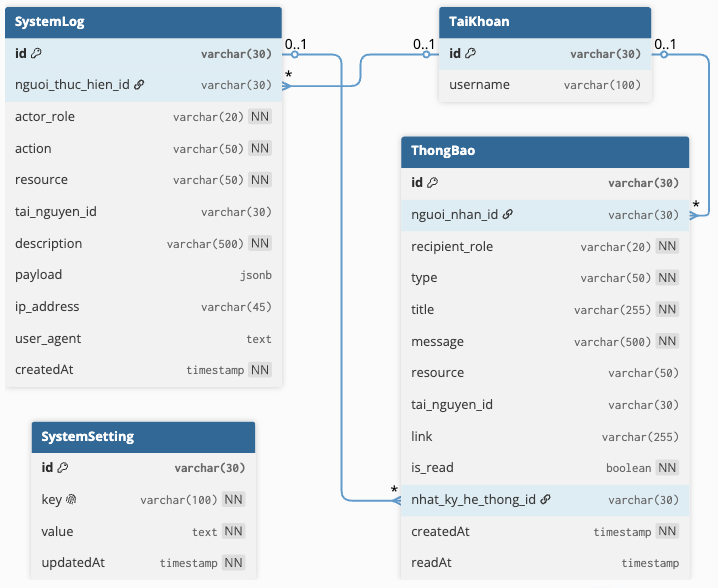
\includegraphics[width=\textwidth,height=0.5\textheight,keepaspectratio]{erd-6-he-thong}\\[0.05cm]
  \scriptsize\raggedright \textbf{Ba bảng:}
  \begin{itemize}\scriptsize
    \item Mỗi bản ghi \texttt{SystemLog} gắn với \texttt{TaiKhoan} người thực hiện (có thể trống với thao tác do hệ thống tự chạy).
    \item Mỗi \texttt{ThongBao} gắn với một \texttt{TaiKhoan} người nhận và có thể trỏ ngược về bản ghi \texttt{SystemLog} đã sinh ra nó.
    \item \texttt{SystemSetting} lưu cấu hình dạng khoá--giá trị, độc lập, không có khoá ngoại.
  \end{itemize}
\end{frame}

% --- Use-case diagram tổng quát ---
\begin{frame}{Biểu đồ use-case tổng quát}
  \centering
  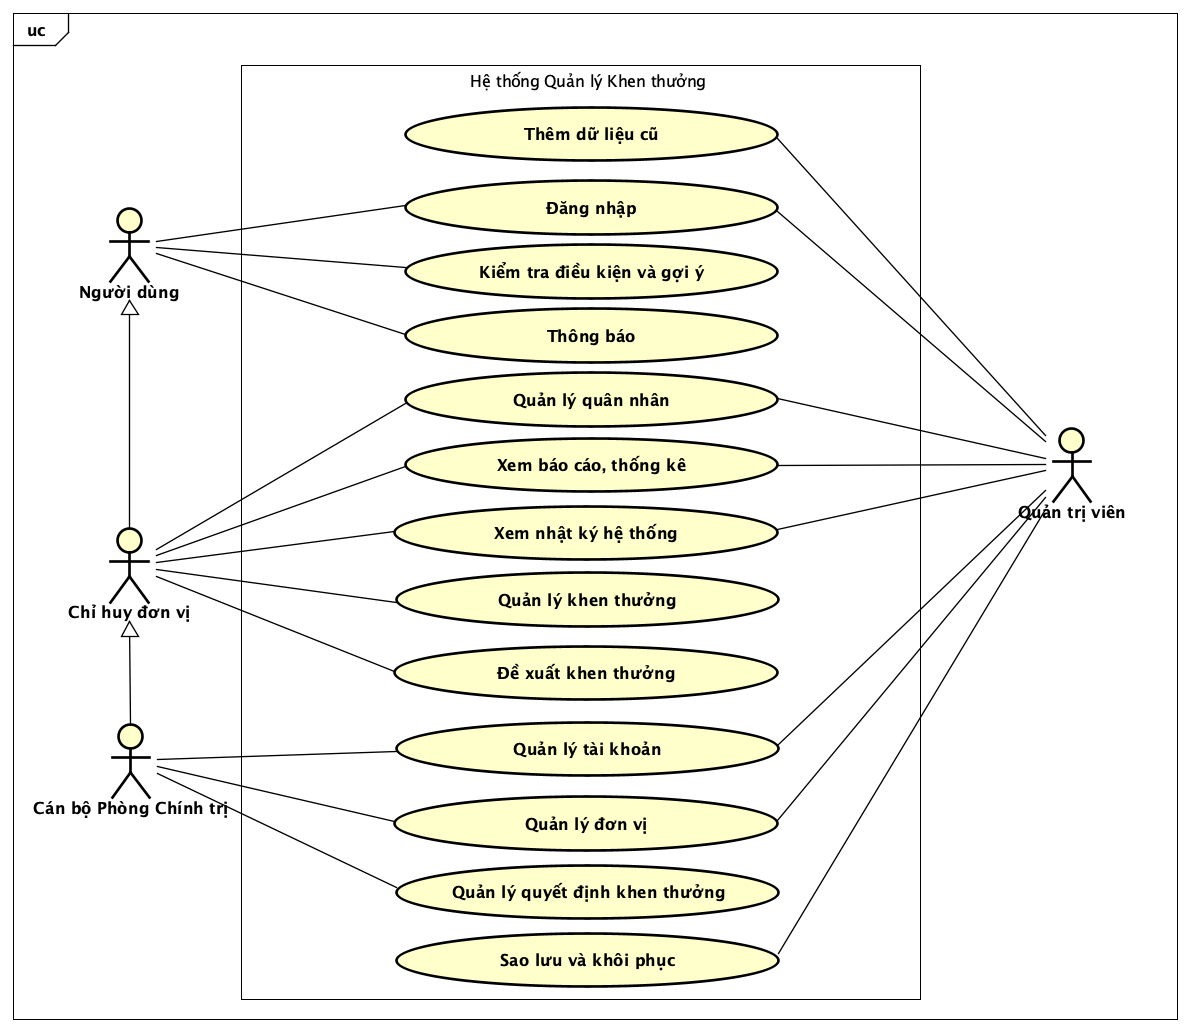
\includegraphics[width=\textwidth,height=0.84\textheight,keepaspectratio]{uc-tong-quan}
\end{frame}

% --- Slide 12: Activity Diagram quy trình duyệt ---
\begin{frame}{Thiết kế hoạt động --- Quy trình duyệt đề xuất}
  \begin{columns}[T,onlytextwidth]
    \column{0.55\textwidth}
    \textbf{Các bước chính}\\[0.2cm]
    \footnotesize
    \begin{enumerate}
      \item Chỉ huy đơn vị tạo đề xuất qua biểu mẫu năm bước
      \item Hệ thống kiểm tra điều kiện, cảnh báo trùng đề xuất
      \item Cán bộ Phòng Chính trị đối chiếu, nhập số quyết định và phê duyệt
      \item Đính kèm tệp PDF quyết định đã ký, lưu kèm bản ghi
      \item Cập nhật hồ sơ, gửi thông báo, ghi nhật ký
    \end{enumerate}
    \vspace{0.2cm}
    \begin{block}{Tính nhất quán}
      \scriptsize Bước 3--5 thực hiện trong \textbf{một transaction Prisma} bảo đảm tính nhất quán của dữ liệu.
    \end{block}

    \column{0.42\textwidth}
    \centering
    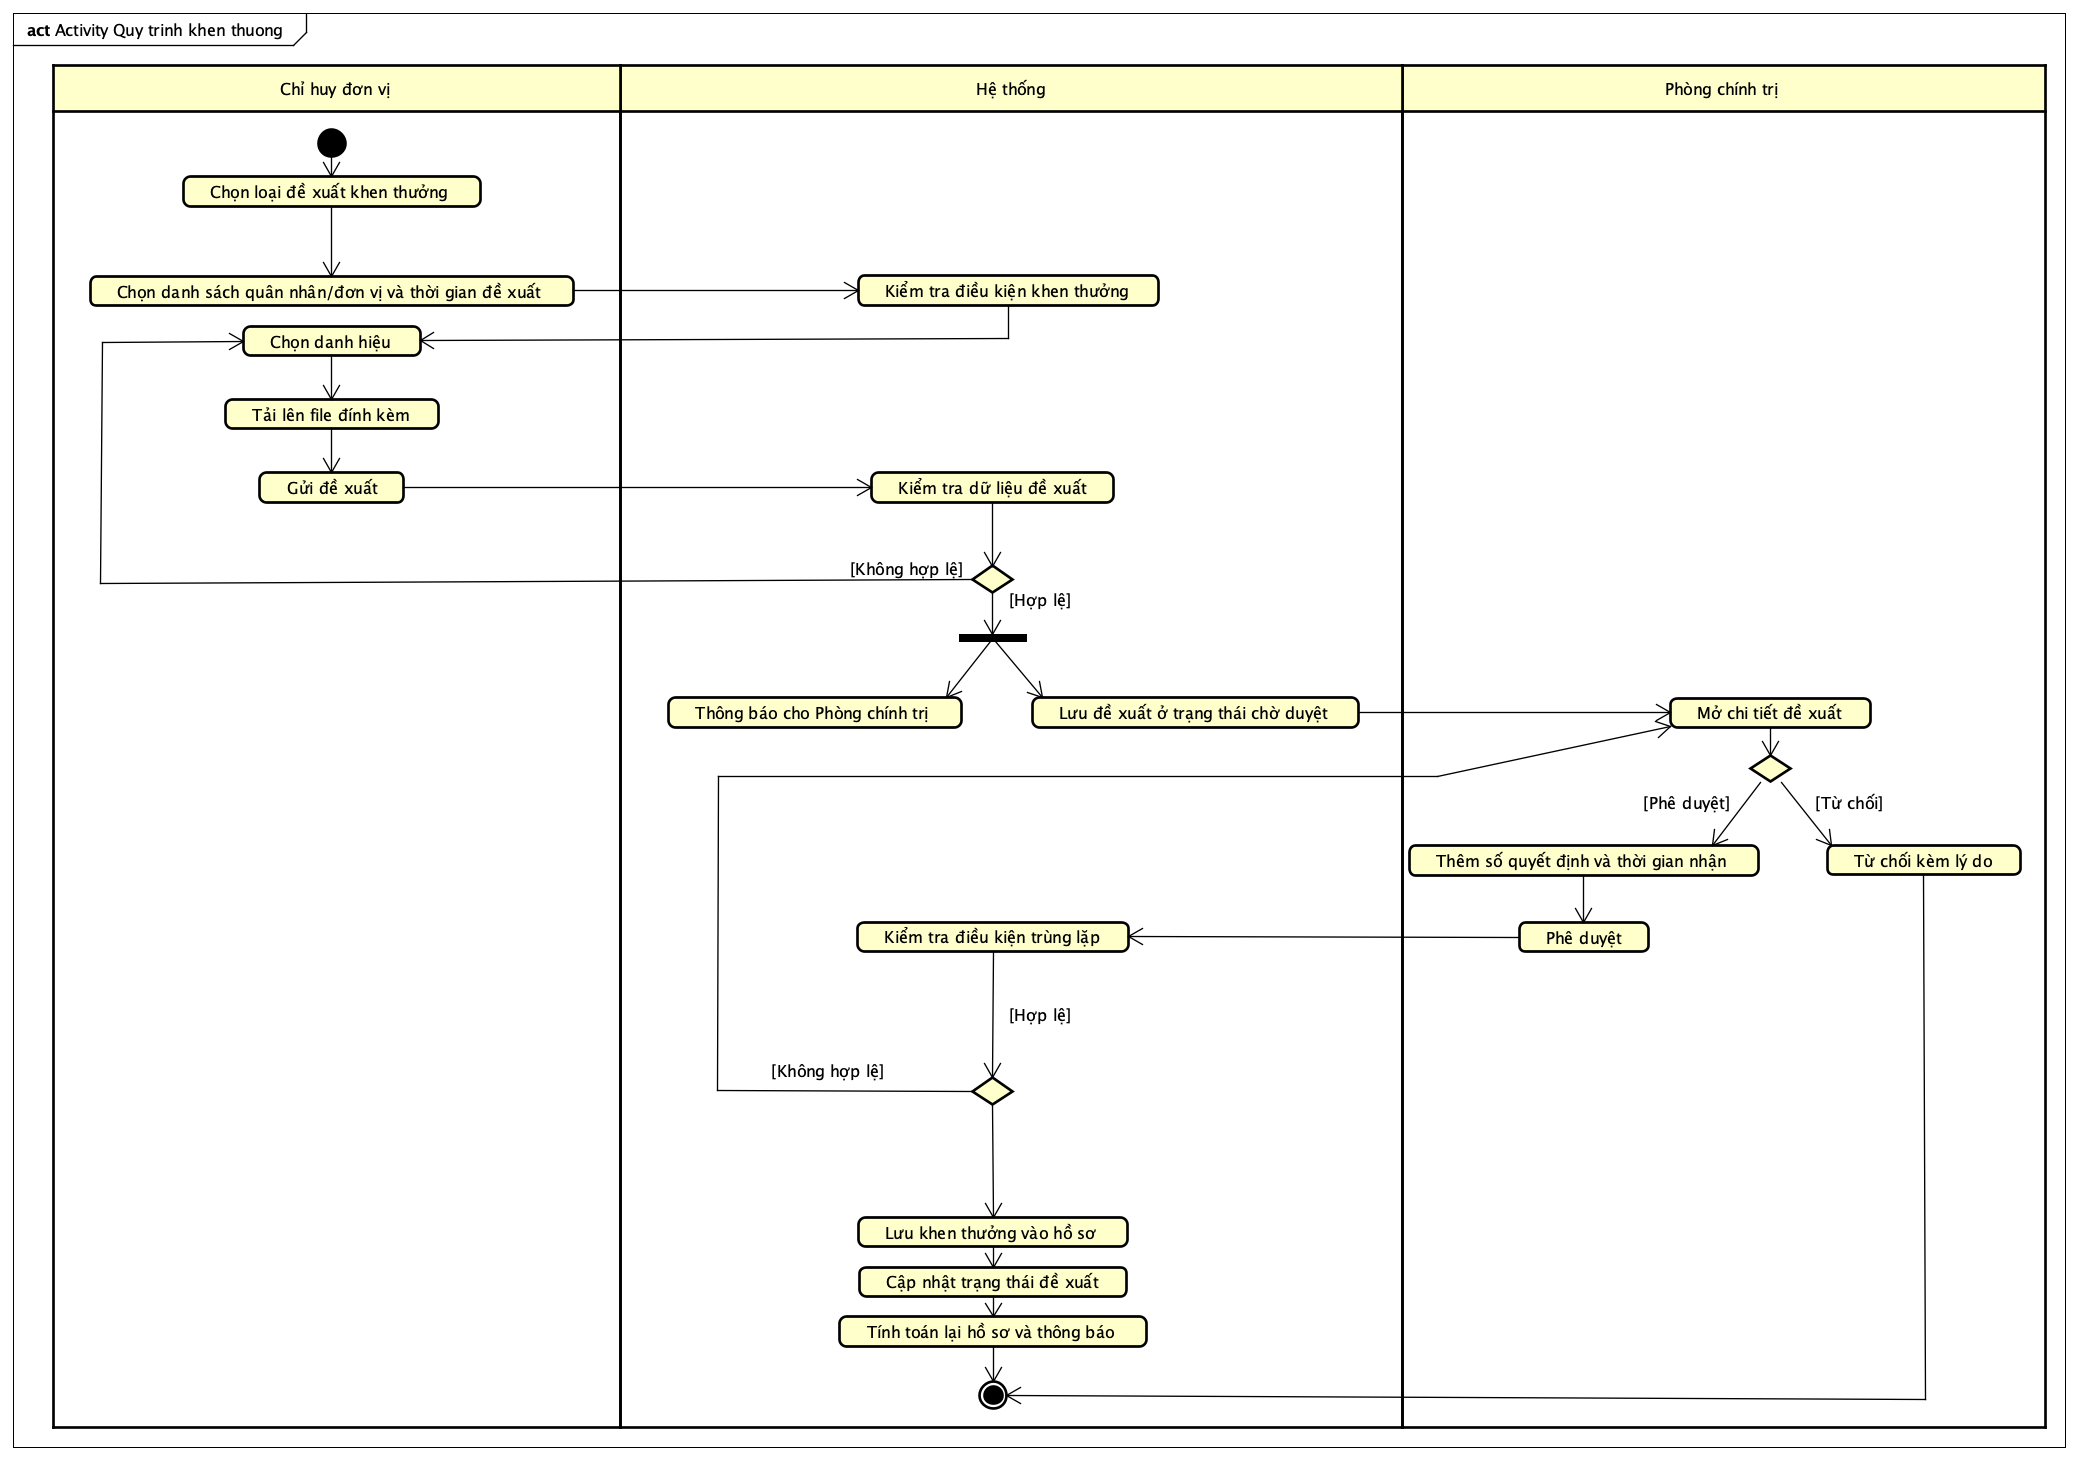
\includegraphics[width=\textwidth,height=0.8\textheight,keepaspectratio]{activity-quy-trinh}
  \end{columns}
\end{frame}

% --- Slide 13: Strategy Pattern ⭐ ---
\begin{frame}[fragile]{Kiến trúc phần mềm --- Strategy Pattern}
  \begin{columns}[T,onlytextwidth]
    \column{0.5\textwidth}
    \textbf{Vấn đề}\\
    \scriptsize Bảy loại đề xuất, mỗi loại có logic submit/validate/import khác nhau $\to$ \texttt{if/else} sẽ tạo file 2000+ dòng, khó test và bảo trì.\\[0.3cm]

    \textbf{Giải pháp}\\
    \scriptsize Định nghĩa \textbf{interface chung}, mỗi loại 1 file riêng, dispatch qua \textbf{Registry}.

    \begin{lstlisting}[basicstyle=\ttfamily\tiny\color{textmain}]
interface ProposalStrategy {
  buildSubmitPayload(data);
  validateApprove(ctx);
  importInTransaction(tx);
  buildSuccessMessage(result);
}
    \end{lstlisting}

    \column{0.5\textwidth}
    \begin{block}{7 Strategy implementations}
      \scriptsize\centering
      \textbf{\textcolor{hustred}{ProposalStrategy}} \textit{(interface)}\\[0.2cm]
      $\swarrow \quad \downarrow \quad \searrow$\\[0.2cm]
      \begin{tabular}{ll}
        caNhanHangNam & donViHangNam \\
        hccsvv & hcbvtq \\
        hcqkqt & knc \\
        \multicolumn{2}{c}{nckh} \\
      \end{tabular}
    \end{block}

    \begin{block}{DRY \& mở rộng}
      \scriptsize HCQKQT và KNC dùng chung một hàm nhập để tránh trùng lặp. \textbf{Kết quả:} thêm loại đề xuất mới chỉ cần một tệp chiến lược và một dòng đăng ký, không phải sửa tầng phê duyệt chung.
    \end{block}
  \end{columns}
\end{frame}

% --- Biểu đồ lớp module đề xuất (Strategy) ---
\begin{frame}{Biểu đồ lớp module đề xuất (Strategy)}
  \centering
  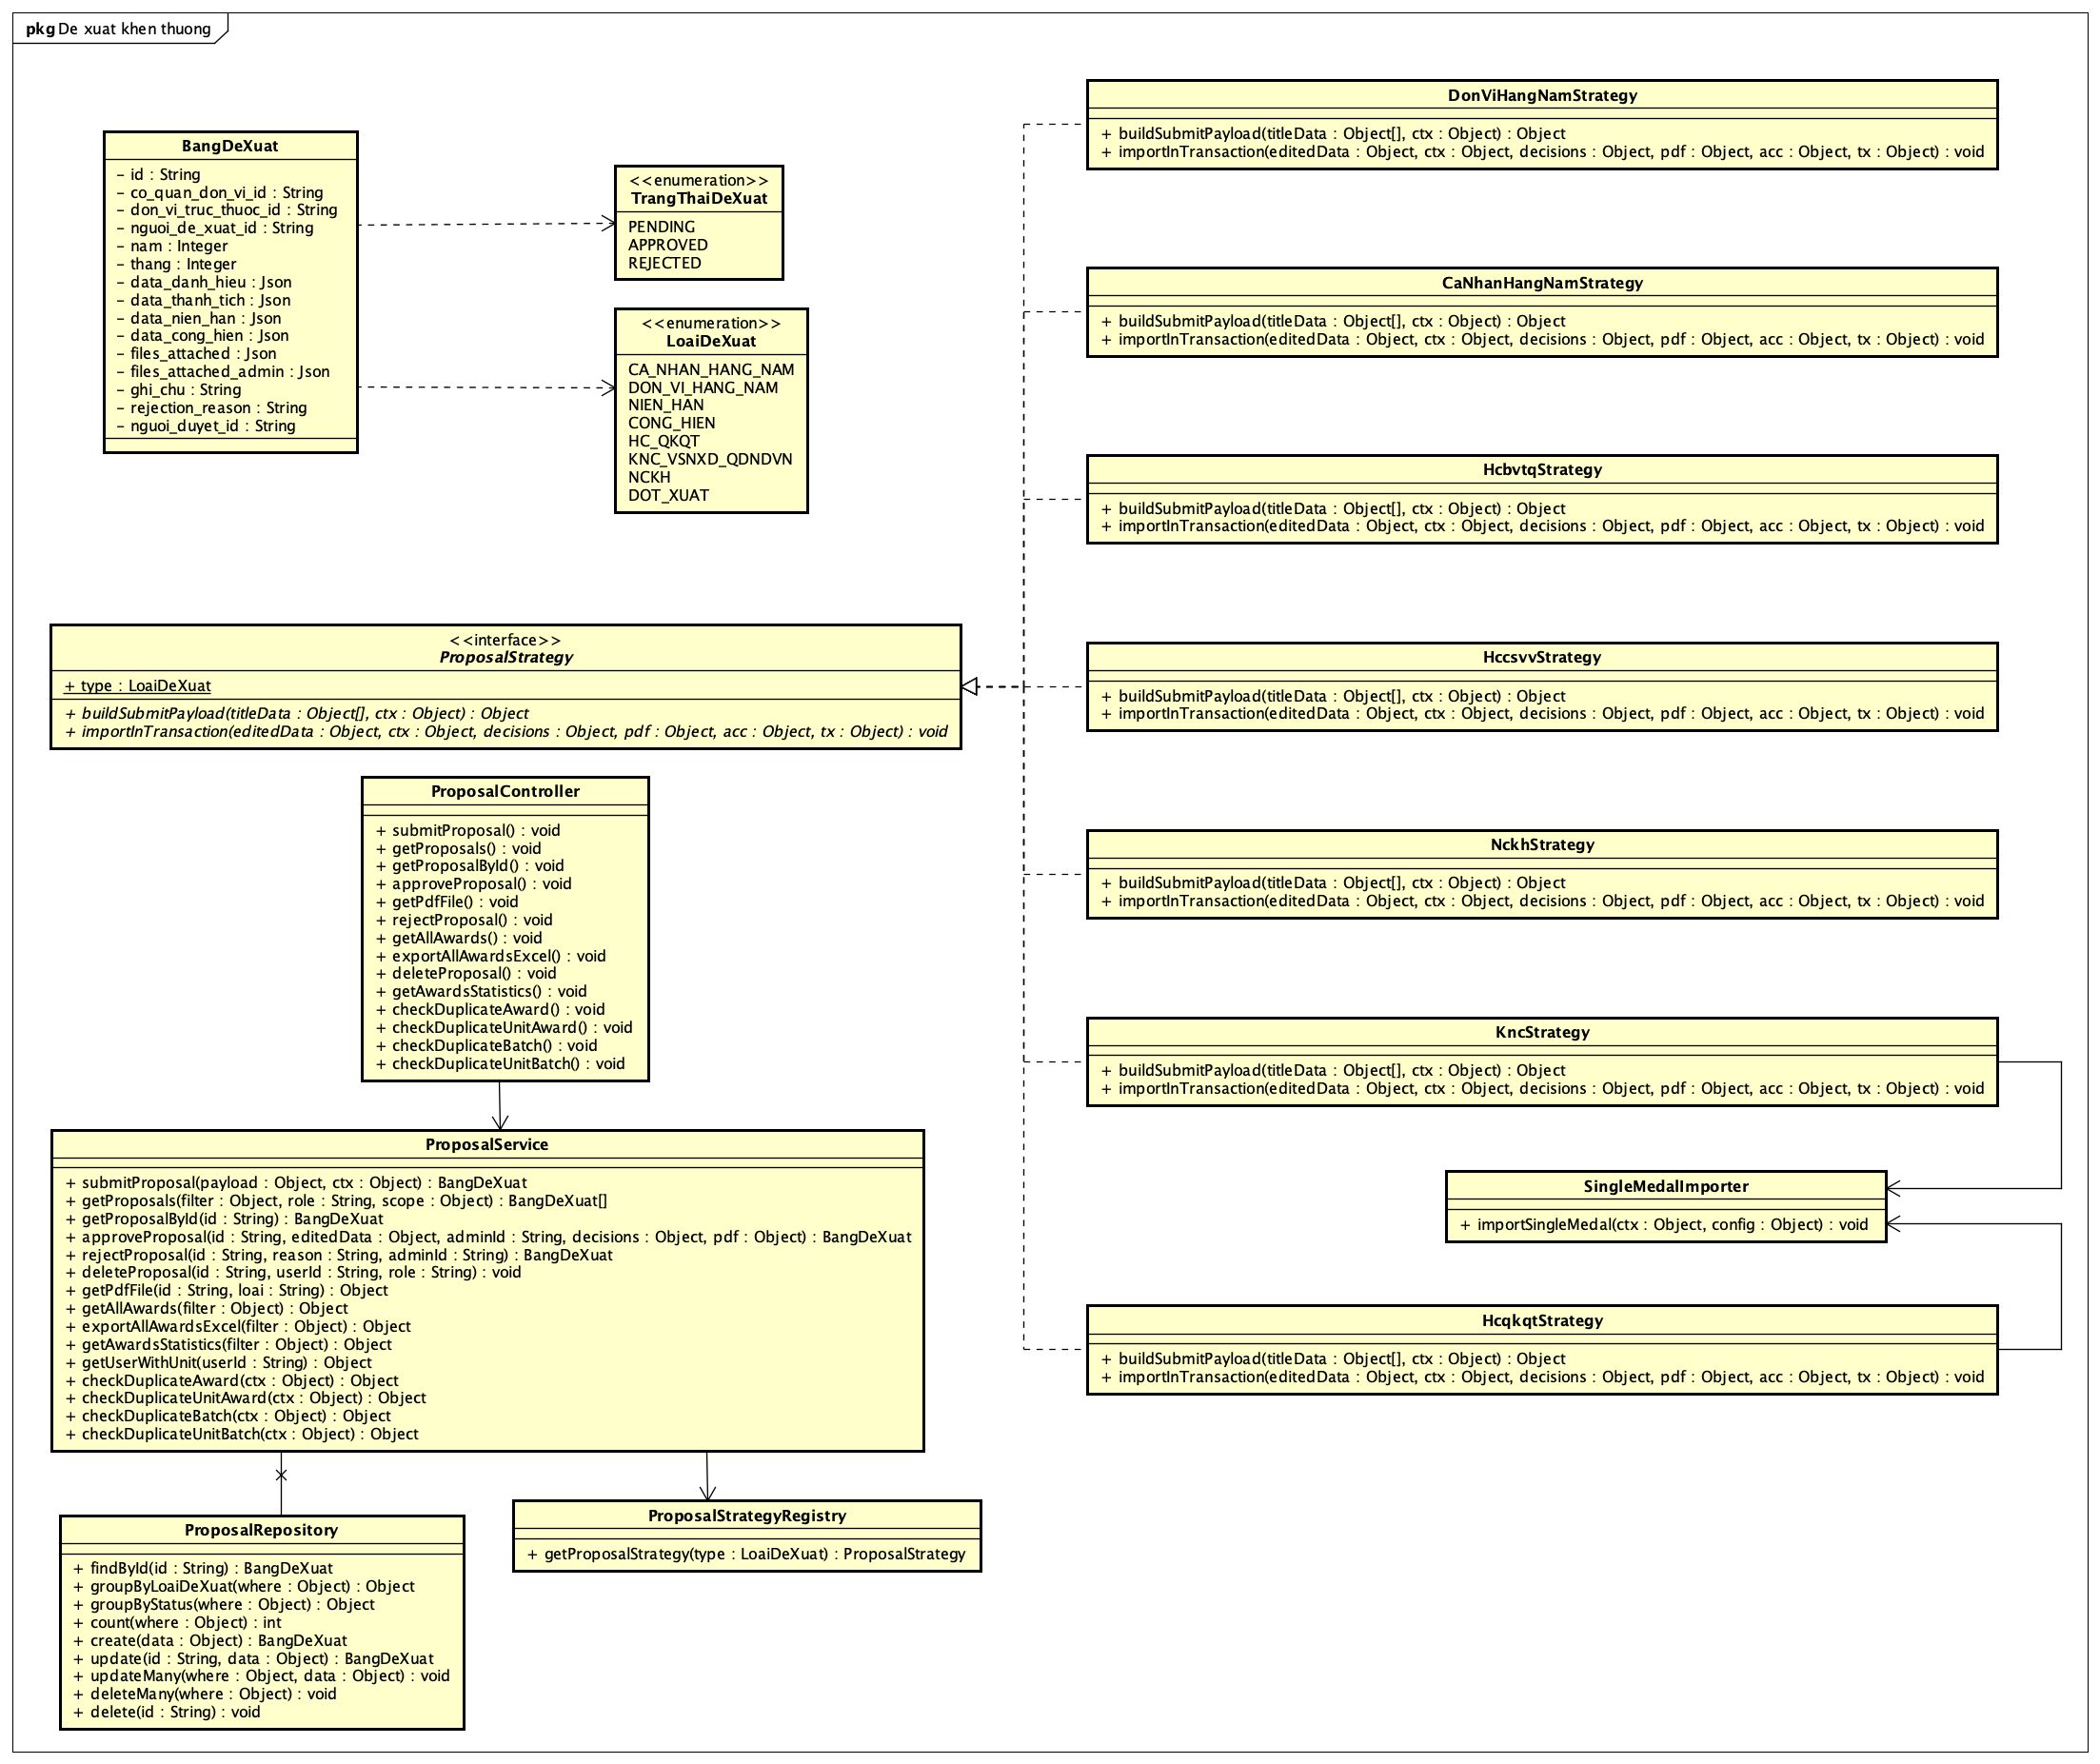
\includegraphics[width=\textwidth,height=0.84\textheight,keepaspectratio]{lop-de-xuat}
\end{frame}

% --- Đóng góp 1: Tự động xét điều kiện & gợi ý ---
\begin{frame}{Tự động xét điều kiện \& gợi ý chủ động}
  \footnotesize
  \textbf{\textcolor{hustred}{Vấn đề}}
  \begin{itemize}\scriptsize
    \item Xét chuỗi danh hiệu thủ công: cửa sổ trượt 3 năm và 7 năm, đếm số BKBTBQP/CSTĐTQ, kiểm NCKH từng năm $\to$ tốn thời gian, dễ tính nhầm và bỏ sót.
  \end{itemize}

  \textbf{\textcolor{hustred}{Cách làm}}
  \begin{itemize}\scriptsize
    \item Mỗi cấp danh hiệu mô tả bằng một dòng cấu hình: chu kỳ, cờ tiền điều kiện, yêu cầu NCKH, nhận một lần duy nhất hay lặp lại.
    \item Một hàm thuần đọc cấu hình và ngữ cảnh chuỗi của quân nhân, trả về kết luận đủ/chưa đủ kèm lý do.
    \item Cùng một bộ quy tắc dùng cho cả tính lại hồ sơ lẫn kiểm tra khi phê duyệt $\to$ hai luồng không lệch nhau.
    \item Tự tính lại khi dữ liệu nguồn thay đổi; tự sinh gợi ý theo năm (vd ``Đủ điều kiện đề nghị BKBTBQP 2026'').
  \end{itemize}

  \textbf{\textcolor{hustred}{Kết quả}}
  \begin{itemize}\scriptsize
    \item Thời gian xét mỗi quân nhân giảm từ vài chục phút xuống gần như tức thời.
    \item Phát hiện đúng cả trường hợp lỡ đợt và quân nhân đủ điều kiện nhưng dễ bị bỏ sót.
  \end{itemize}
\end{frame}

% --- Đóng góp 2: Số hoá quy trình đề xuất & lưu vết ---
\begin{frame}{Số hoá quy trình đề xuất \& lưu vết thao tác}
  \footnotesize
  \textbf{\textcolor{hustred}{Vấn đề}}
  \begin{itemize}\scriptsize
    \item Quy trình giấy nhiều bước (đơn vị lập $\to$ Phòng Chính trị tổng hợp $\to$ Ban Giám đốc duyệt) kéo dài 5--10 ngày.
    \item Chỉnh sửa giữa chừng chỉ ghi tay trên bản nháp $\to$ không truy được ai sửa, sửa gì, vì sao.
  \end{itemize}

  \textbf{\textcolor{hustred}{Cách làm}}
  \begin{itemize}\scriptsize
    \item Đề xuất là một thực thể có ba trạng thái (chờ duyệt / đã duyệt / từ chối); bảy loại đi theo cùng một giao diện chung.
    \item Chỉ huy đơn vị tạo đề xuất, Cán bộ Phòng Chính trị duyệt hoặc từ chối kèm lý do; biểu mẫu xác thực bằng schema Zod dùng chung hai phía.
    \item Trước khi duyệt, cán bộ nhập số quyết định và đính kèm tệp PDF quyết định đã ký; sau đó thao tác phê duyệt gói trong một giao dịch: ghi danh hiệu, gắn quyết định, đổi trạng thái; xong mới tính lại hồ sơ và ghi nhật ký.
  \end{itemize}

  \textbf{\textcolor{hustred}{Kết quả}}
  \begin{itemize}\scriptsize
    \item Rút thời gian một đợt xét từ nhiều ngày xuống trong ngày.
    \item Truy vết trọn vòng đời một đề xuất (từ chối $\to$ đề nghị lại $\to$ duyệt) kèm người thực hiện, thời điểm và lý do.
  \end{itemize}
\end{frame}

% --- Đóng góp 3: Nhập Excel hàng loạt có giao dịch ---
\begin{frame}{Nhập Excel hàng loạt có giao dịch \& kiểm tra trước}
  \footnotesize
  \textbf{\textcolor{hustred}{Vấn đề}}
  \begin{itemize}\scriptsize
    \item Di trú dữ liệu lịch sử lớn (ước tính khoảng 50.000 bản ghi danh hiệu và 15.000 lịch sử chức vụ) từ tệp Word và bản giấy.
    \item Nhập tay mất nhiều tháng; chạy thẳng câu lệnh SQL rủi ro toàn vẹn vì định dạng nguồn không thống nhất.
  \end{itemize}

  \textbf{\textcolor{hustred}{Cách làm}}
  \begin{itemize}\scriptsize
    \item Quy trình hai bước: \textbf{Xem trước} đối chiếu schema Zod và quy tắc nghiệp vụ, liệt kê từng dòng lỗi nhưng chưa ghi xuống cơ sở dữ liệu.
    \item \textbf{Xác nhận} ghi tuần tự trong một giao dịch; lỗi ở bất kỳ dòng nào thì hoàn tác toàn bộ.
    \item Tệp mẫu có danh sách thả xuống (Data Validation); tự chuẩn hoá nhiều biến thể viết tắt danh hiệu về một mã chuẩn.
  \end{itemize}

  \textbf{\textcolor{hustred}{Kết quả}}
  \begin{itemize}\scriptsize
    \item Di trú khối dữ liệu lớn trong thời gian ngắn; không bản ghi nào lọt vào ở trạng thái dở dang.
    \item Hỗ trợ thêm xuất danh sách khen thưởng ra Excel theo năm và theo đơn vị.
  \end{itemize}
\end{frame}

% --- Đóng góp 4: Lưu vết, sao lưu & thông báo ---
\begin{frame}{Lưu vết đầy đủ, sao lưu định kỳ \& thông báo}
  \footnotesize
  \textbf{\textcolor{hustred}{Vấn đề}}
  \begin{itemize}\scriptsize
    \item Tệp dùng chung chỉ kiểm soát ở mức thư mục; sửa hay xoá không để lại dấu vết.
    \item Sao lưu phụ thuộc kỷ luật cá nhân, không bảo đảm luôn có bản gần nhất để khôi phục.
  \end{itemize}

  \textbf{\textcolor{hustred}{Cách làm}}
  \begin{itemize}\scriptsize
    \item Nhật ký hệ thống ghi mọi thao tác đổi dữ liệu: người thực hiện, hành động, đối tượng, địa chỉ IP và dữ liệu trước/sau; lọc đa chiều.
    \item Sao lưu định kỳ tự động bằng \texttt{node-cron}, kết xuất tệp SQL và dọn bản cũ; lịch cấu hình trong khu vực DevZone.
    \item Thông báo thời gian thực qua Socket.IO theo từng người nhận, đồng thời lưu vào bảng \texttt{ThongBao} để xem lại khi đăng nhập.
  \end{itemize}

  \textbf{\textcolor{hustred}{Kết quả}}
  \begin{itemize}\scriptsize
    \item Mọi thay đổi dữ liệu đều truy vết được; nhật ký sao lưu chỉ Quản trị hệ thống xem được.
    \item Luôn có bản sao lưu hằng ngày sẵn sàng khôi phục, không phụ thuộc thao tác thủ công.
  \end{itemize}
\end{frame}

% --- Slide 18: Kiểm thử + Hiệu năng + Triển khai ⭐ ---
\begin{frame}{Kiểm thử, Hiệu năng và Triển khai}
  \begin{columns}[T,onlytextwidth]
    \column{0.55\textwidth}
    \textbf{Kiểm thử}\\[0.2cm]

    \begin{block}{Hai hướng bổ trợ}
      \scriptsize Kiểm thử \textbf{hộp đen thủ công} qua giao diện (tám nhóm chức năng nghiệp vụ) kết hợp kiểm thử \textbf{tự động bằng Jest} cho các quy tắc xét chuỗi lõi; thêm kiểm thử tương thích trên năm dòng máy và bốn trình duyệt.
    \end{block}

    \scriptsize\textbf{Một số kịch bản trọng yếu:}
    \begin{enumerate}\scriptsize
      \item \textbf{Tranh chấp ghi} --- hai cán bộ duyệt cùng lúc, chỉ một thành công
      \item \textbf{Xét điều kiện BKTTCP} --- cửa sổ trượt 7 năm + ràng buộc một lần duy nhất
      \item \textbf{Chống giả mạo} --- gửi thẳng dữ liệu sai qua API, backend vẫn xét lại và từ chối
      \item \textbf{Lỡ đợt} --- bỏ lỡ mốc đề nghị, chu kỳ sau vẫn được xét đúng
    \end{enumerate}

    \column{0.4\textwidth}
    \textbf{Triển khai mạng nội bộ}\\[0.2cm]
    \scriptsize
    \begin{enumerate}
      \item Chuẩn bị máy chủ Windows Server (Node.js 20 LTS, PostgreSQL 15)
      \item Cấu hình \texttt{.env}; chạy \texttt{prisma migrate dev} tạo lược đồ và khởi tạo tài khoản Quản trị hệ thống
      \item \texttt{pm2 start ecosystem.config.js} chạy backend (cổng 4000) và frontend (cổng 3000); \texttt{pm2 save} để tự khởi động cùng máy
    \end{enumerate}

    \begin{block}{Vận hành}
      \scriptsize PM2 tự khởi động lại khi tiến trình lỗi và ghi log có thời gian. Hệ thống chạy \textbf{hoàn toàn trong mạng nội bộ}, không phụ thuộc Internet.
    \end{block}
  \end{columns}
\end{frame}

% --- Slide 19: Kết luận và Hướng phát triển ---
\begin{frame}{Kết luận và hướng phát triển}
  \begin{columns}[T,onlytextwidth]
    \column{0.33\textwidth}
    \textbf{\textcolor{hustred}{Đã đạt được}}
    \begin{itemize}\scriptsize
      \item Hoàn thành bảy nhóm khen thưởng, 4 vai trò
      \item Tự động hoá quy trình xét duyệt
      \item Kiểm thử kỹ các kịch bản nghiệp vụ trọng yếu
      \item Triển khai trên mạng nội bộ
      \item Layered + Strategy pattern
    \end{itemize}

    \column{0.33\textwidth}
    \textbf{\textcolor{hustred}{Hạn chế}}
    \begin{itemize}\scriptsize
      \item BKTTCP cá nhân lifetime --- chưa hỗ trợ danh hiệu cao hơn
      \item Chưa có module BI thống kê chi tiết
      \item Chỉ chạy 1 instance --- chưa scale ngang
      \item Ký số còn dưới dạng file PDF
    \end{itemize}

    \column{0.33\textwidth}
    \textbf{\textcolor{hustred}{Hướng phát triển}}
    \begin{itemize}\scriptsize
      \item Ứng dụng di động cho cấp duyệt nhanh
      \item Module BI: biểu đồ xu hướng theo năm \& đơn vị
      \item Tích hợp \textbf{Smart Card / USB token}
      \item Cluster mode + Redis adapter Socket.IO
    \end{itemize}
  \end{columns}

  \vspace{0.3cm}
  \begin{block}{}
    \centering\small Phần mềm đã sẵn sàng \highlight{triển khai thử nghiệm tại đơn vị}, đáp ứng đầy đủ các mục tiêu đặt ra ban đầu.
  \end{block}
\end{frame}

% --- Slide 20: Cảm ơn ---
{
\setbeamertemplate{footline}{}
\begin{frame}[plain]
  \begin{center}
    \vspace{1.5cm}
    {\huge \textcolor{hustred}{\textbf{EM XIN TRÂN TRỌNG CẢM ƠN}}}\\[1cm]

    {\Large Hội đồng đã lắng nghe phần trình bày}\\[1.5cm]

    {\large Em rất mong nhận được \highlight{nhận xét và câu hỏi} từ Hội đồng}\\[2cm]

    {\Huge \textcolor{hustred}{$\heartsuit$}}\\
    {\Large \textcolor{hustdark}{Q\&A}}
  \end{center}
\end{frame}
}

\end{document}
